\documentclass[twoside]{book}

% Packages required by doxygen
\usepackage{calc}
\usepackage{doxygen}
\usepackage{graphicx}
\usepackage[utf8]{inputenc}
\usepackage{makeidx}
\usepackage{multicol}
\usepackage{multirow}
\usepackage{textcomp}
\usepackage[table]{xcolor}

% Font selection
\usepackage[T1]{fontenc}
\usepackage{mathptmx}
\usepackage[scaled=.90]{helvet}
\usepackage{courier}
\usepackage{amssymb}
\usepackage{sectsty}
\renewcommand{\familydefault}{\sfdefault}
\allsectionsfont{%
  \fontseries{bc}\selectfont%
  \color{darkgray}%
}
\renewcommand{\DoxyLabelFont}{%
  \fontseries{bc}\selectfont%
  \color{darkgray}%
}

% Page & text layout
\usepackage{geometry}
\geometry{%
  a4paper,%
  top=2.5cm,%
  bottom=2.5cm,%
  left=2.5cm,%
  right=2.5cm%
}
\tolerance=750
\hfuzz=15pt
\hbadness=750
\setlength{\emergencystretch}{15pt}
\setlength{\parindent}{0cm}
\setlength{\parskip}{0.2cm}
\makeatletter
\renewcommand{\paragraph}{%
  \@startsection{paragraph}{4}{0ex}{-1.0ex}{1.0ex}{%
    \normalfont\normalsize\bfseries\SS@parafont%
  }%
}
\renewcommand{\subparagraph}{%
  \@startsection{subparagraph}{5}{0ex}{-1.0ex}{1.0ex}{%
    \normalfont\normalsize\bfseries\SS@subparafont%
  }%
}
\makeatother

% Headers & footers
\usepackage{fancyhdr}
\pagestyle{fancyplain}
\fancyhead[LE]{\fancyplain{}{\bfseries\thepage}}
\fancyhead[CE]{\fancyplain{}{}}
\fancyhead[RE]{\fancyplain{}{\bfseries\leftmark}}
\fancyhead[LO]{\fancyplain{}{\bfseries\rightmark}}
\fancyhead[CO]{\fancyplain{}{}}
\fancyhead[RO]{\fancyplain{}{\bfseries\thepage}}
\fancyfoot[LE]{\fancyplain{}{}}
\fancyfoot[CE]{\fancyplain{}{}}
\fancyfoot[RE]{\fancyplain{}{\bfseries\scriptsize Generated on Wed Sep 30 2015 16\-:51\-:23 for Greenfeed -\/ E\-M\-S\-E server program by Doxygen }}
\fancyfoot[LO]{\fancyplain{}{\bfseries\scriptsize Generated on Wed Sep 30 2015 16\-:51\-:23 for Greenfeed -\/ E\-M\-S\-E server program by Doxygen }}
\fancyfoot[CO]{\fancyplain{}{}}
\fancyfoot[RO]{\fancyplain{}{}}
\renewcommand{\footrulewidth}{0.4pt}
\renewcommand{\chaptermark}[1]{%
  \markboth{#1}{}%
}
\renewcommand{\sectionmark}[1]{%
  \markright{\thesection\ #1}%
}

% Indices & bibliography
\usepackage{natbib}
\usepackage[titles]{tocloft}
\setcounter{tocdepth}{3}
\setcounter{secnumdepth}{5}
\makeindex

% Hyperlinks (required, but should be loaded last)
\usepackage{ifpdf}
\ifpdf
  \usepackage[pdftex,pagebackref=true]{hyperref}
\else
  \usepackage[ps2pdf,pagebackref=true]{hyperref}
\fi
\hypersetup{%
  colorlinks=true,%
  linkcolor=blue,%
  citecolor=blue,%
  unicode%
}

% Custom commands
\newcommand{\clearemptydoublepage}{%
  \newpage{\pagestyle{empty}\cleardoublepage}%
}


%===== C O N T E N T S =====

\begin{document}

% Titlepage & ToC
\hypersetup{pageanchor=false}
\pagenumbering{roman}
\begin{titlepage}
\vspace*{7cm}
\begin{center}%
{\Large Greenfeed -\/ E\-M\-S\-E server program \\[1ex]\large 1.\-0 }\\
\vspace*{1cm}
{\large Generated by Doxygen 1.8.6}\\
\vspace*{0.5cm}
{\small Wed Sep 30 2015 16:51:23}\\
\end{center}
\end{titlepage}
\clearemptydoublepage
\tableofcontents
\clearemptydoublepage
\pagenumbering{arabic}
\hypersetup{pageanchor=true}

%--- Begin generated contents ---
\chapter{Data Structure Index}
\section{Data Structures}
Here are the data structures with brief descriptions\-:\begin{DoxyCompactList}
\item\contentsline{section}{\hyperlink{structbase64__decodestate}{base64\-\_\-decodestate} }{\pageref{structbase64__decodestate}}{}
\item\contentsline{section}{\hyperlink{structbase64_1_1base64__decodestate}{base64\-\_\-decodestate} }{\pageref{structbase64_1_1base64__decodestate}}{}
\item\contentsline{section}{\hyperlink{structbase64__encodestate}{base64\-\_\-encodestate} }{\pageref{structbase64__encodestate}}{}
\item\contentsline{section}{\hyperlink{structbase64_1_1base64__encodestate}{base64\-\_\-encodestate} }{\pageref{structbase64_1_1base64__encodestate}}{}
\item\contentsline{section}{\hyperlink{structbase64_1_1decoder}{decoder} }{\pageref{structbase64_1_1decoder}}{}
\item\contentsline{section}{\hyperlink{structdownstream__packet}{downstream\-\_\-packet} \\*This structure represents a package that must be sent to the Io\-T station to make it send a Lo\-Ra message Some of these fields are optional }{\pageref{structdownstream__packet}}{}
\item\contentsline{section}{\hyperlink{structbase64_1_1encoder}{encoder} }{\pageref{structbase64_1_1encoder}}{}
\item\contentsline{section}{\hyperlink{unioniot__pull__data}{iot\-\_\-pull\-\_\-data} }{\pageref{unioniot__pull__data}}{}
\item\contentsline{section}{\hyperlink{unioniot__push__data}{iot\-\_\-push\-\_\-data} \\*To have more information about this structure, look at the \hyperlink{unioniot__pull__data}{iot\-\_\-pull\-\_\-data} }{\pageref{unioniot__push__data}}{}
\item\contentsline{section}{\hyperlink{structiot__stat}{iot\-\_\-stat} }{\pageref{structiot__stat}}{}
\item\contentsline{section}{\hyperlink{structjson__array__t}{json\-\_\-array\-\_\-t} }{\pageref{structjson__array__t}}{}
\item\contentsline{section}{\hyperlink{structjson__object__t}{json\-\_\-object\-\_\-t} }{\pageref{structjson__object__t}}{}
\item\contentsline{section}{\hyperlink{structjson__value__t}{json\-\_\-value\-\_\-t} }{\pageref{structjson__value__t}}{}
\item\contentsline{section}{\hyperlink{unionjson__value__value}{json\-\_\-value\-\_\-value} }{\pageref{unionjson__value__value}}{}
\item\contentsline{section}{\hyperlink{structpull__resp}{pull\-\_\-resp} }{\pageref{structpull__resp}}{}
\item\contentsline{section}{\hyperlink{structrxpk}{rxpk} }{\pageref{structrxpk}}{}
\item\contentsline{section}{\hyperlink{structupstream__packet}{upstream\-\_\-packet} }{\pageref{structupstream__packet}}{}
\end{DoxyCompactList}

\chapter{File Index}
\section{File List}
Here is a list of all documented files with brief descriptions\-:\begin{DoxyCompactList}
\item\contentsline{section}{\hyperlink{main_8c}{main.\-c} \\*This file is the entry of the main program to communicate with the Kerlink Io\-T station }{\pageref{main_8c}}{}
\item\contentsline{section}{includes/\hyperlink{constants_8h}{constants.\-h} \\*This file defines some constants used in the program }{\pageref{constants_8h}}{}
\item\contentsline{section}{includes/\hyperlink{downstream__packet_8h}{downstream\-\_\-packet.\-h} \\*This file defines the structure \char`\"{}downstream\-\_\-packet\char`\"{} }{\pageref{downstream__packet_8h}}{}
\item\contentsline{section}{includes/\hyperlink{iot__pull__data_8h}{iot\-\_\-pull\-\_\-data.\-h} \\*This file defines a structure used to represent the pull\-\_\-data message sent by the Io\-T station }{\pageref{iot__pull__data_8h}}{}
\item\contentsline{section}{includes/\hyperlink{iot__push__data_8h}{iot\-\_\-push\-\_\-data.\-h} \\*This file defines a structure used to represent the push\-\_\-data message sent by the Io\-T station }{\pageref{iot__push__data_8h}}{}
\item\contentsline{section}{includes/\hyperlink{manage__downstream_8h}{manage\-\_\-downstream.\-h} \\*This file defines some function prototypes and global variables }{\pageref{manage__downstream_8h}}{}
\item\contentsline{section}{includes/\hyperlink{manage__upstream_8h}{manage\-\_\-upstream.\-h} \\*This file defines some function prototypes and global variables }{\pageref{manage__upstream_8h}}{}
\item\contentsline{section}{includes/\hyperlink{types_8h}{types.\-h} \\*This file defines some typedef }{\pageref{types_8h}}{}
\item\contentsline{section}{includes/{\bfseries upstream\-\_\-packet.\-h} }{\pageref{upstream__packet_8h}}{}
\item\contentsline{section}{includes/b64/{\bfseries cdecode.\-h} }{\pageref{cdecode_8h}}{}
\item\contentsline{section}{includes/b64/{\bfseries cencode.\-h} }{\pageref{cencode_8h}}{}
\item\contentsline{section}{includes/b64/{\bfseries decode.\-h} }{\pageref{decode_8h}}{}
\item\contentsline{section}{includes/b64/{\bfseries encode.\-h} }{\pageref{encode_8h}}{}
\item\contentsline{section}{parson/{\bfseries parson.\-h} }{\pageref{parson_8h}}{}
\end{DoxyCompactList}

\chapter{Data Structure Documentation}
\hypertarget{structbase64__decodestate}{\section{base64\-\_\-decodestate Struct Reference}
\label{structbase64__decodestate}\index{base64\-\_\-decodestate@{base64\-\_\-decodestate}}
}
\subsection*{Data Fields}
\begin{DoxyCompactItemize}
\item 
\hypertarget{structbase64__decodestate_a448927d59479ddab147ed380104d2cbe}{base64\-\_\-decodestep {\bfseries step}}\label{structbase64__decodestate_a448927d59479ddab147ed380104d2cbe}

\item 
\hypertarget{structbase64__decodestate_ad1b3e9f303925389dcd09100288913d4}{char {\bfseries plainchar}}\label{structbase64__decodestate_ad1b3e9f303925389dcd09100288913d4}

\end{DoxyCompactItemize}


The documentation for this struct was generated from the following file\-:\begin{DoxyCompactItemize}
\item 
includes/b64/cdecode.\-h\end{DoxyCompactItemize}

\hypertarget{structbase64_1_1base64__decodestate}{\section{base64\-\_\-decodestate Struct Reference}
\label{structbase64_1_1base64__decodestate}\index{base64\-\_\-decodestate@{base64\-\_\-decodestate}}
}
\subsection*{Data Fields}
\begin{DoxyCompactItemize}
\item 
\hypertarget{structbase64_1_1base64__decodestate_a448927d59479ddab147ed380104d2cbe}{base64\-\_\-decodestep {\bfseries step}}\label{structbase64_1_1base64__decodestate_a448927d59479ddab147ed380104d2cbe}

\item 
\hypertarget{structbase64_1_1base64__decodestate_ad1b3e9f303925389dcd09100288913d4}{char {\bfseries plainchar}}\label{structbase64_1_1base64__decodestate_ad1b3e9f303925389dcd09100288913d4}

\end{DoxyCompactItemize}


The documentation for this struct was generated from the following file\-:\begin{DoxyCompactItemize}
\item 
includes/b64/decode.\-h\end{DoxyCompactItemize}

\hypertarget{structbase64__encodestate}{\section{base64\-\_\-encodestate Struct Reference}
\label{structbase64__encodestate}\index{base64\-\_\-encodestate@{base64\-\_\-encodestate}}
}
\subsection*{Data Fields}
\begin{DoxyCompactItemize}
\item 
\hypertarget{structbase64__encodestate_a03379869bcae52baa816bfb820a526d2}{base64\-\_\-encodestep {\bfseries step}}\label{structbase64__encodestate_a03379869bcae52baa816bfb820a526d2}

\item 
\hypertarget{structbase64__encodestate_a53ba5e5a2744d7ec9192157fc755a94d}{char {\bfseries result}}\label{structbase64__encodestate_a53ba5e5a2744d7ec9192157fc755a94d}

\item 
\hypertarget{structbase64__encodestate_abaa3aa9865cb2e6be3da3d466554c0b5}{int {\bfseries stepcount}}\label{structbase64__encodestate_abaa3aa9865cb2e6be3da3d466554c0b5}

\end{DoxyCompactItemize}


The documentation for this struct was generated from the following file\-:\begin{DoxyCompactItemize}
\item 
includes/b64/cencode.\-h\end{DoxyCompactItemize}

\hypertarget{structbase64_1_1base64__encodestate}{\section{base64\-\_\-encodestate Struct Reference}
\label{structbase64_1_1base64__encodestate}\index{base64\-\_\-encodestate@{base64\-\_\-encodestate}}
}
\subsection*{Data Fields}
\begin{DoxyCompactItemize}
\item 
\hypertarget{structbase64_1_1base64__encodestate_a03379869bcae52baa816bfb820a526d2}{base64\-\_\-encodestep {\bfseries step}}\label{structbase64_1_1base64__encodestate_a03379869bcae52baa816bfb820a526d2}

\item 
\hypertarget{structbase64_1_1base64__encodestate_a53ba5e5a2744d7ec9192157fc755a94d}{char {\bfseries result}}\label{structbase64_1_1base64__encodestate_a53ba5e5a2744d7ec9192157fc755a94d}

\item 
\hypertarget{structbase64_1_1base64__encodestate_abaa3aa9865cb2e6be3da3d466554c0b5}{int {\bfseries stepcount}}\label{structbase64_1_1base64__encodestate_abaa3aa9865cb2e6be3da3d466554c0b5}

\end{DoxyCompactItemize}


The documentation for this struct was generated from the following file\-:\begin{DoxyCompactItemize}
\item 
includes/b64/encode.\-h\end{DoxyCompactItemize}

\hypertarget{structbase64_1_1decoder}{\section{decoder Struct Reference}
\label{structbase64_1_1decoder}\index{decoder@{decoder}}
}


Collaboration diagram for decoder\-:\nopagebreak
\begin{figure}[H]
\begin{center}
\leavevmode
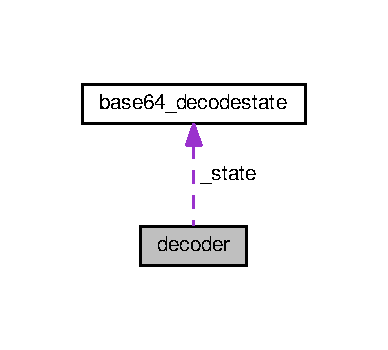
\includegraphics[width=186pt]{structbase64_1_1decoder__coll__graph}
\end{center}
\end{figure}
\subsection*{Public Member Functions}
\begin{DoxyCompactItemize}
\item 
\hypertarget{structbase64_1_1decoder_afb1a3c0484762c72b2c1a9500a30f63a}{{\bfseries decoder} (int buffersize\-\_\-in=B\-U\-F\-F\-E\-R\-S\-I\-Z\-E)}\label{structbase64_1_1decoder_afb1a3c0484762c72b2c1a9500a30f63a}

\item 
\hypertarget{structbase64_1_1decoder_a6542188945ec1885416c0725ab0b9e11}{int {\bfseries decode} (char value\-\_\-in)}\label{structbase64_1_1decoder_a6542188945ec1885416c0725ab0b9e11}

\item 
\hypertarget{structbase64_1_1decoder_ae569f424cafa612fd0871f0d7f0b433a}{int {\bfseries decode} (const char $\ast$code\-\_\-in, const int length\-\_\-in, char $\ast$plaintext\-\_\-out)}\label{structbase64_1_1decoder_ae569f424cafa612fd0871f0d7f0b433a}

\item 
\hypertarget{structbase64_1_1decoder_a02f06a7109ed4e6da96350242f5051b2}{void {\bfseries decode} (std\-::istream \&istream\-\_\-in, std\-::ostream \&ostream\-\_\-in)}\label{structbase64_1_1decoder_a02f06a7109ed4e6da96350242f5051b2}

\end{DoxyCompactItemize}
\subsection*{Data Fields}
\begin{DoxyCompactItemize}
\item 
\hypertarget{structbase64_1_1decoder_acf9f75b5896098cd4cec6524f798be71}{\hyperlink{structbase64_1_1base64__decodestate}{base64\-\_\-decodestate} {\bfseries \-\_\-state}}\label{structbase64_1_1decoder_acf9f75b5896098cd4cec6524f798be71}

\item 
\hypertarget{structbase64_1_1decoder_ab9ef2d501bcca4a9f9e076df6044201c}{int {\bfseries \-\_\-buffersize}}\label{structbase64_1_1decoder_ab9ef2d501bcca4a9f9e076df6044201c}

\end{DoxyCompactItemize}


The documentation for this struct was generated from the following file\-:\begin{DoxyCompactItemize}
\item 
includes/b64/decode.\-h\end{DoxyCompactItemize}

\hypertarget{structdownstream__packet}{\section{downstream\-\_\-packet Struct Reference}
\label{structdownstream__packet}\index{downstream\-\_\-packet@{downstream\-\_\-packet}}
}


This structure represents a package that must be sent to the Io\-T station to make it send a Lo\-Ra message Some of these fields are optional.  




{\ttfamily \#include $<$includes/downstream\-\_\-packet.\-h$>$}

\subsection*{Data Fields}
\begin{DoxyCompactItemize}
\item 
bool \hyperlink{structdownstream__packet_a2233496db347682f0b4005fe07310c58}{send\-\_\-now}
\item 
long \hyperlink{structdownstream__packet_ac5deed89768140dbc80dbc6529a5e14a}{timestamp}
\item 
char \hyperlink{structdownstream__packet_a7ba42be95635137cb867f08c8aa01f3b}{time} \mbox{[}35\mbox{]}
\item 
double \hyperlink{structdownstream__packet_a4c45cdff103e6644a620ba5061509f22}{frequency}
\item 
unsigned int \hyperlink{structdownstream__packet_a566a9646361d592aa0be3fe468b29aad}{rf\-\_\-channel}
\item 
unsigned int \hyperlink{structdownstream__packet_a59104ad6aeccc2a5011202486a11959f}{power}
\item 
char \hyperlink{structdownstream__packet_a167264916b5fad13dd3dc470128e3eef}{modulation} \mbox{[}5\mbox{]}
\item 
char \hyperlink{structdownstream__packet_a96f84d084cdf0e910c2482be0632fa97}{datarate} \mbox{[}15\mbox{]}
\item 
unsigned int \hyperlink{structdownstream__packet_ae4bd55e8e15052cb4ac21a9aba5866ad}{fsk\-\_\-datarate}
\item 
char \hyperlink{structdownstream__packet_a9bb17e8dc14670aedcd5b69e797d19d7}{code\-\_\-rate} \mbox{[}10\mbox{]}
\item 
unsigned int \hyperlink{structdownstream__packet_a3f5d6010dd5bdc3cedcb44caece43a59}{fsk\-\_\-deviation}
\item 
bool \hyperlink{structdownstream__packet_a17de42e009f605885975928f7dad2d0c}{i\-\_\-polarization}
\item 
unsigned int \hyperlink{structdownstream__packet_a4f552d54b9b164e0e8677ba5e591c84c}{rf\-\_\-preamble}
\item 
unsigned int \hyperlink{structdownstream__packet_a75b5ec600c45b3430f28b8bcf16d868a}{payload\-\_\-size}
\item 
char $\ast$ \hyperlink{structdownstream__packet_a91a70b77df95bd8b0830b49a094c2acb}{data}
\item 
bool \hyperlink{structdownstream__packet_af235dcb1657075c3d7f13390ee408eea}{disable\-\_\-\-C\-R\-C}
\end{DoxyCompactItemize}


\subsection{Detailed Description}
This structure represents a package that must be sent to the Io\-T station to make it send a Lo\-Ra message Some of these fields are optional. 

\subsection{Field Documentation}
\hypertarget{structdownstream__packet_a9bb17e8dc14670aedcd5b69e797d19d7}{\index{downstream\-\_\-packet@{downstream\-\_\-packet}!code\-\_\-rate@{code\-\_\-rate}}
\index{code\-\_\-rate@{code\-\_\-rate}!downstream_packet@{downstream\-\_\-packet}}
\subsubsection[{code\-\_\-rate}]{\setlength{\rightskip}{0pt plus 5cm}char code\-\_\-rate\mbox{[}10\mbox{]}}}\label{structdownstream__packet_a9bb17e8dc14670aedcd5b69e797d19d7}
The code rate used to emit the packet, example 4/5 \hypertarget{structdownstream__packet_a91a70b77df95bd8b0830b49a094c2acb}{\index{downstream\-\_\-packet@{downstream\-\_\-packet}!data@{data}}
\index{data@{data}!downstream_packet@{downstream\-\_\-packet}}
\subsubsection[{data}]{\setlength{\rightskip}{0pt plus 5cm}char$\ast$ data}}\label{structdownstream__packet_a91a70b77df95bd8b0830b49a094c2acb}
The actual payload in base64 \hypertarget{structdownstream__packet_a96f84d084cdf0e910c2482be0632fa97}{\index{downstream\-\_\-packet@{downstream\-\_\-packet}!datarate@{datarate}}
\index{datarate@{datarate}!downstream_packet@{downstream\-\_\-packet}}
\subsubsection[{datarate}]{\setlength{\rightskip}{0pt plus 5cm}char datarate\mbox{[}15\mbox{]}}}\label{structdownstream__packet_a96f84d084cdf0e910c2482be0632fa97}
The datarate used in case the L\-O\-R\-A modulation is chosen \hypertarget{structdownstream__packet_af235dcb1657075c3d7f13390ee408eea}{\index{downstream\-\_\-packet@{downstream\-\_\-packet}!disable\-\_\-\-C\-R\-C@{disable\-\_\-\-C\-R\-C}}
\index{disable\-\_\-\-C\-R\-C@{disable\-\_\-\-C\-R\-C}!downstream_packet@{downstream\-\_\-packet}}
\subsubsection[{disable\-\_\-\-C\-R\-C}]{\setlength{\rightskip}{0pt plus 5cm}bool disable\-\_\-\-C\-R\-C}}\label{structdownstream__packet_af235dcb1657075c3d7f13390ee408eea}
If this field is set to true, the C\-R\-C check will be disabled (should always be set to false!) \hypertarget{structdownstream__packet_a4c45cdff103e6644a620ba5061509f22}{\index{downstream\-\_\-packet@{downstream\-\_\-packet}!frequency@{frequency}}
\index{frequency@{frequency}!downstream_packet@{downstream\-\_\-packet}}
\subsubsection[{frequency}]{\setlength{\rightskip}{0pt plus 5cm}double frequency}}\label{structdownstream__packet_a4c45cdff103e6644a620ba5061509f22}
The central frequency used when the packet is emitted \hypertarget{structdownstream__packet_ae4bd55e8e15052cb4ac21a9aba5866ad}{\index{downstream\-\_\-packet@{downstream\-\_\-packet}!fsk\-\_\-datarate@{fsk\-\_\-datarate}}
\index{fsk\-\_\-datarate@{fsk\-\_\-datarate}!downstream_packet@{downstream\-\_\-packet}}
\subsubsection[{fsk\-\_\-datarate}]{\setlength{\rightskip}{0pt plus 5cm}unsigned int fsk\-\_\-datarate}}\label{structdownstream__packet_ae4bd55e8e15052cb4ac21a9aba5866ad}
The datarate used in case the F\-S\-K modulation is chosen \hypertarget{structdownstream__packet_a3f5d6010dd5bdc3cedcb44caece43a59}{\index{downstream\-\_\-packet@{downstream\-\_\-packet}!fsk\-\_\-deviation@{fsk\-\_\-deviation}}
\index{fsk\-\_\-deviation@{fsk\-\_\-deviation}!downstream_packet@{downstream\-\_\-packet}}
\subsubsection[{fsk\-\_\-deviation}]{\setlength{\rightskip}{0pt plus 5cm}unsigned int fsk\-\_\-deviation}}\label{structdownstream__packet_a3f5d6010dd5bdc3cedcb44caece43a59}
The F\-S\-K frequency deviation \hypertarget{structdownstream__packet_a17de42e009f605885975928f7dad2d0c}{\index{downstream\-\_\-packet@{downstream\-\_\-packet}!i\-\_\-polarization@{i\-\_\-polarization}}
\index{i\-\_\-polarization@{i\-\_\-polarization}!downstream_packet@{downstream\-\_\-packet}}
\subsubsection[{i\-\_\-polarization}]{\setlength{\rightskip}{0pt plus 5cm}bool i\-\_\-polarization}}\label{structdownstream__packet_a17de42e009f605885975928f7dad2d0c}
If this field is set to true, the Lo\-Ra modulation polarization will be inversed \hypertarget{structdownstream__packet_a167264916b5fad13dd3dc470128e3eef}{\index{downstream\-\_\-packet@{downstream\-\_\-packet}!modulation@{modulation}}
\index{modulation@{modulation}!downstream_packet@{downstream\-\_\-packet}}
\subsubsection[{modulation}]{\setlength{\rightskip}{0pt plus 5cm}char modulation\mbox{[}5\mbox{]}}}\label{structdownstream__packet_a167264916b5fad13dd3dc470128e3eef}
The Lo\-Ra modulation used\-: L\-O\-R\-A or F\-S\-K. Other values will be discarded \hypertarget{structdownstream__packet_a75b5ec600c45b3430f28b8bcf16d868a}{\index{downstream\-\_\-packet@{downstream\-\_\-packet}!payload\-\_\-size@{payload\-\_\-size}}
\index{payload\-\_\-size@{payload\-\_\-size}!downstream_packet@{downstream\-\_\-packet}}
\subsubsection[{payload\-\_\-size}]{\setlength{\rightskip}{0pt plus 5cm}unsigned int payload\-\_\-size}}\label{structdownstream__packet_a75b5ec600c45b3430f28b8bcf16d868a}
The payload size in bytes \hypertarget{structdownstream__packet_a59104ad6aeccc2a5011202486a11959f}{\index{downstream\-\_\-packet@{downstream\-\_\-packet}!power@{power}}
\index{power@{power}!downstream_packet@{downstream\-\_\-packet}}
\subsubsection[{power}]{\setlength{\rightskip}{0pt plus 5cm}unsigned int power}}\label{structdownstream__packet_a59104ad6aeccc2a5011202486a11959f}
The power used by the antenna to emit the packet \hypertarget{structdownstream__packet_a566a9646361d592aa0be3fe468b29aad}{\index{downstream\-\_\-packet@{downstream\-\_\-packet}!rf\-\_\-channel@{rf\-\_\-channel}}
\index{rf\-\_\-channel@{rf\-\_\-channel}!downstream_packet@{downstream\-\_\-packet}}
\subsubsection[{rf\-\_\-channel}]{\setlength{\rightskip}{0pt plus 5cm}unsigned int rf\-\_\-channel}}\label{structdownstream__packet_a566a9646361d592aa0be3fe468b29aad}
The channel the Io\-T station will use to emit the packet \hypertarget{structdownstream__packet_a4f552d54b9b164e0e8677ba5e591c84c}{\index{downstream\-\_\-packet@{downstream\-\_\-packet}!rf\-\_\-preamble@{rf\-\_\-preamble}}
\index{rf\-\_\-preamble@{rf\-\_\-preamble}!downstream_packet@{downstream\-\_\-packet}}
\subsubsection[{rf\-\_\-preamble}]{\setlength{\rightskip}{0pt plus 5cm}unsigned int rf\-\_\-preamble}}\label{structdownstream__packet_a4f552d54b9b164e0e8677ba5e591c84c}
The R\-F preamble size \hypertarget{structdownstream__packet_a2233496db347682f0b4005fe07310c58}{\index{downstream\-\_\-packet@{downstream\-\_\-packet}!send\-\_\-now@{send\-\_\-now}}
\index{send\-\_\-now@{send\-\_\-now}!downstream_packet@{downstream\-\_\-packet}}
\subsubsection[{send\-\_\-now}]{\setlength{\rightskip}{0pt plus 5cm}bool send\-\_\-now}}\label{structdownstream__packet_a2233496db347682f0b4005fe07310c58}
If this field is equal to true, the packet will be sent by the Io\-T station immediately \hypertarget{structdownstream__packet_a7ba42be95635137cb867f08c8aa01f3b}{\index{downstream\-\_\-packet@{downstream\-\_\-packet}!time@{time}}
\index{time@{time}!downstream_packet@{downstream\-\_\-packet}}
\subsubsection[{time}]{\setlength{\rightskip}{0pt plus 5cm}char time\mbox{[}35\mbox{]}}}\label{structdownstream__packet_a7ba42be95635137cb867f08c8aa01f3b}
Same use that the timestamp field. The representation of the date is different \hypertarget{structdownstream__packet_ac5deed89768140dbc80dbc6529a5e14a}{\index{downstream\-\_\-packet@{downstream\-\_\-packet}!timestamp@{timestamp}}
\index{timestamp@{timestamp}!downstream_packet@{downstream\-\_\-packet}}
\subsubsection[{timestamp}]{\setlength{\rightskip}{0pt plus 5cm}long timestamp}}\label{structdownstream__packet_ac5deed89768140dbc80dbc6529a5e14a}
If the send\-\_\-now field is set to false, the packet will be sent when the current date of the Io\-T station reaches this value 

The documentation for this struct was generated from the following file\-:\begin{DoxyCompactItemize}
\item 
includes/\hyperlink{downstream__packet_8h}{downstream\-\_\-packet.\-h}\end{DoxyCompactItemize}

\hypertarget{structbase64_1_1encoder}{\section{encoder Struct Reference}
\label{structbase64_1_1encoder}\index{encoder@{encoder}}
}


Collaboration diagram for encoder\-:\nopagebreak
\begin{figure}[H]
\begin{center}
\leavevmode
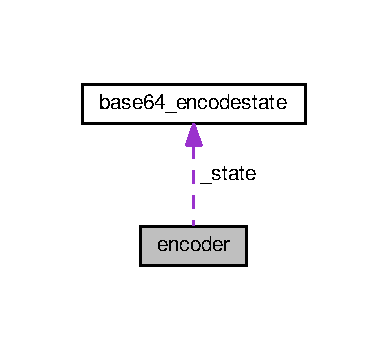
\includegraphics[width=186pt]{structbase64_1_1encoder__coll__graph}
\end{center}
\end{figure}
\subsection*{Public Member Functions}
\begin{DoxyCompactItemize}
\item 
\hypertarget{structbase64_1_1encoder_a53baabc4bbcd1213330c98579e5ad0a2}{{\bfseries encoder} (int buffersize\-\_\-in=B\-U\-F\-F\-E\-R\-S\-I\-Z\-E)}\label{structbase64_1_1encoder_a53baabc4bbcd1213330c98579e5ad0a2}

\item 
\hypertarget{structbase64_1_1encoder_ae38a98a537afc3e6952a15d01d3d074d}{int {\bfseries encode} (char value\-\_\-in)}\label{structbase64_1_1encoder_ae38a98a537afc3e6952a15d01d3d074d}

\item 
\hypertarget{structbase64_1_1encoder_a5676f45347ba7ca994d4493c278060e7}{int {\bfseries encode} (const char $\ast$code\-\_\-in, const int length\-\_\-in, char $\ast$plaintext\-\_\-out)}\label{structbase64_1_1encoder_a5676f45347ba7ca994d4493c278060e7}

\item 
\hypertarget{structbase64_1_1encoder_a694bb20cc355b5ed33358970a9b4c615}{int {\bfseries encode\-\_\-end} (char $\ast$plaintext\-\_\-out)}\label{structbase64_1_1encoder_a694bb20cc355b5ed33358970a9b4c615}

\item 
\hypertarget{structbase64_1_1encoder_a3b48510504ae53d21173c22cf6f32ca9}{void {\bfseries encode} (std\-::istream \&istream\-\_\-in, std\-::ostream \&ostream\-\_\-in)}\label{structbase64_1_1encoder_a3b48510504ae53d21173c22cf6f32ca9}

\end{DoxyCompactItemize}
\subsection*{Data Fields}
\begin{DoxyCompactItemize}
\item 
\hypertarget{structbase64_1_1encoder_a229a86fbbf4f36949427ef5c29a77e5e}{\hyperlink{structbase64_1_1base64__encodestate}{base64\-\_\-encodestate} {\bfseries \-\_\-state}}\label{structbase64_1_1encoder_a229a86fbbf4f36949427ef5c29a77e5e}

\item 
\hypertarget{structbase64_1_1encoder_ab9ef2d501bcca4a9f9e076df6044201c}{int {\bfseries \-\_\-buffersize}}\label{structbase64_1_1encoder_ab9ef2d501bcca4a9f9e076df6044201c}

\end{DoxyCompactItemize}


The documentation for this struct was generated from the following file\-:\begin{DoxyCompactItemize}
\item 
includes/b64/encode.\-h\end{DoxyCompactItemize}

\hypertarget{unioniot__pull__data}{\section{iot\-\_\-pull\-\_\-data Union Reference}
\label{unioniot__pull__data}\index{iot\-\_\-pull\-\_\-data@{iot\-\_\-pull\-\_\-data}}
}


{\ttfamily \#include \char`\"{}includes/iot\-\_\-pull\-\_\-data.\-h\char`\"{}}

\subsection*{Data Fields}
\begin{DoxyCompactItemize}
\item 
char \hyperlink{unioniot__pull__data_a019f7d47cfe35a4e91ae5068647c1014}{msg} \mbox{[}\hyperlink{constants_8h_a786442238545011e2a0eb7ce468ad692}{I\-N\-C\-O\-M\-M\-I\-N\-G\-\_\-\-M\-S\-G\-\_\-\-S\-I\-Z\-E}\mbox{]}
\item 
\hypertarget{unioniot__pull__data_a4aedf31c3dc77c1995181f8ac4236ff0}{\begin{tabbing}
xx\=xx\=xx\=xx\=xx\=xx\=xx\=xx\=xx\=\kill
struct \{\\
\>byte \hyperlink{unioniot__pull__data_a4723ed0bc6ed806bf66757d25e40641a}{protocol\_version}\\
\hypertarget{structiot__pull__data_1_1@0_ada15cc4b0b6fe37df4be93e5260089e3}{\>byte {\bfseries token} \mbox{[}2\mbox{]}\\
\hypertarget{structiot__pull__data_1_1@0_a3661902d618d08427f1ab8cca0411413}{\>byte {\bfseries pull\_data\_id}\\
\hypertarget{structiot__pull__data_1_1@0_a7badc8040877155f12b7d17871dfe626}{\>byte {\bfseries MAC} \mbox{[}8\mbox{]}\\
\hypertarget{structiot__pull__data_1_1@0_a95fd1d801d35ecbda7a3a9b479d2d2f3}{\>char {\bfseries json} \mbox{[}\hyperlink{constants_8h_a786442238545011e2a0eb7ce468ad692}{INCOMMING\_MSG\_SIZE}-\/1-\/2-\/1-\/8\mbox{]}\\
\}; }\label{unioniot__pull__data_a4aedf31c3dc77c1995181f8ac4236ff0}
\\

\end{tabbing}\end{DoxyCompactItemize}


\subsection{Detailed Description}
Here is a part of the official documentation. The structure \hyperlink{unioniot__pull__data}{iot\-\_\-pull\-\_\-data} is a C representation of the documentation \paragraph*{5.\-2. P\-U\-L\-L\-\_\-\-D\-A\-T\-A packet}

That packet type is used by the gateway to poll data from the server.

This data exchange is initialized by the gateway because it might be impossible for the server to send packets to the gateway if the gateway is behind a N\-A\-T.

When the gateway initialize the exchange, the network route towards the server will open and will allow for packets to flow both directions. The gateway must periodically send P\-U\-L\-L\-\_\-\-D\-A\-T\-A packets to be sure the network route stays open for the server to be used at any time.

\begin{TabularC}{2}
\hline
\rowcolor{lightgray}\PBS\centering {\bf Bytes }&{\bf Function  }\\\cline{1-2}
\PBS\centering 0 &protocol version = 1 \\\cline{1-2}
\PBS\centering 1-\/2 &random token \\\cline{1-2}
\PBS\centering 3 &P\-U\-L\-L\-\_\-\-D\-A\-T\-A identifier 0x02 \\\cline{1-2}
\PBS\centering 4-\/11 &Gateway unique identifier (M\-A\-C address) \\\cline{1-2}
\end{TabularC}
An union is different from a structure in how it manages memory. In a structure, the memory scheme is as follow \-: \par
 $\vert$\-\_\-field A\-\_\-$\vert$\-\_\-\-\_\-\-\_\-\-\_\-\-\_\-\-\_\-\-\_\-\-\_\-\-\_\-\-\_\-\-\_\-\-\_\- field B\-\_\-\-\_\-\-\_\-\-\_\-\-\_\-\-\_\-\-\_\-\-\_\-\-\_\-\-\_\-$\vert$ Padding $\vert$\-\_\-\-\_\-\-\_\-\-\_\-\-Field C\-\_\-\-\_\-\-\_\-\-\_\-$\vert$ ... \par
 Each field starts when the field before stops (some padding may be added, by that's an other topic). An union typical scheme is as follow\-: \par
 $\vert$\-\_\-field A\-\_\-$\vert$\par
 $\vert$\-\_\-\-\_\-\-\_\-\-\_\-\-\_\-\-\_\-\-\_\-\-\_\-\-\_\-\-\_\-\-\_\-field B\-\_\-\-\_\-\-\_\-\-\_\-\-\_\-\-\_\-\-\_\-\-\_\-\-\_\-$\vert$\par
 $\vert$field C$\vert$\par
 All the fields start at the same adress. \par
 So, why an union? As the documentation says, the message received by the server is a 12 bytes, and each byte has its own usage. We have to \char`\"{}cut\char`\"{} the message in part to get each packet of bytes. We could have done it by using the substring function, but that's boring (need to manage memory allocation, calculate indexes ...). By using an union A\-N\-D an internal structure, we can achieve the same thing by way more easily. We use an union to make the message and the internal structure to start at the same address. Then we use the structure memory scheme to create fields which have the perfect size to \char`\"{}cut\char`\"{} the message where it needs to be. Let's see the result \-: \par
 

As we can see, the protocol\-\_\-version field of the structure has the same content of the first byte of the message, and so does token ... 

\subsection{Field Documentation}
\hypertarget{unioniot__pull__data_a019f7d47cfe35a4e91ae5068647c1014}{\index{iot\-\_\-pull\-\_\-data@{iot\-\_\-pull\-\_\-data}!msg@{msg}}
\index{msg@{msg}!iot_pull_data@{iot\-\_\-pull\-\_\-data}}
\subsubsection[{msg}]{\setlength{\rightskip}{0pt plus 5cm}char msg\mbox{[}{\bf I\-N\-C\-O\-M\-M\-I\-N\-G\-\_\-\-M\-S\-G\-\_\-\-S\-I\-Z\-E}\mbox{]}}}\label{unioniot__pull__data_a019f7d47cfe35a4e91ae5068647c1014}
This is the field in which the message sent by the Io\-T station will be \hypertarget{unioniot__pull__data_a4723ed0bc6ed806bf66757d25e40641a}{\index{iot\-\_\-pull\-\_\-data@{iot\-\_\-pull\-\_\-data}!protocol\-\_\-version@{protocol\-\_\-version}}
\index{protocol\-\_\-version@{protocol\-\_\-version}!iot_pull_data@{iot\-\_\-pull\-\_\-data}}
\subsubsection[{protocol\-\_\-version}]{\setlength{\rightskip}{0pt plus 5cm}byte protocol\-\_\-version}}\label{unioniot__pull__data_a4723ed0bc6ed806bf66757d25e40641a}
This is the structure which will cut the message. To have some explanations about the packed attribute, go see Mr L\-A\-L\-E\-V\-E\-E 

The documentation for this union was generated from the following file\-:\begin{DoxyCompactItemize}
\item 
includes/\hyperlink{iot__pull__data_8h}{iot\-\_\-pull\-\_\-data.\-h}\end{DoxyCompactItemize}

\hypertarget{unioniot__push__data}{\section{iot\-\_\-push\-\_\-data Union Reference}
\label{unioniot__push__data}\index{iot\-\_\-push\-\_\-data@{iot\-\_\-push\-\_\-data}}
}


To have more information about this structure, look at the \hyperlink{unioniot__pull__data}{iot\-\_\-pull\-\_\-data}.  




{\ttfamily \#include \char`\"{}includes/iot\-\_\-push\-\_\-data.\-h\char`\"{}}

\subsection*{Data Fields}
\begin{DoxyCompactItemize}
\item 
\hypertarget{unioniot__push__data_a019f7d47cfe35a4e91ae5068647c1014}{char {\bfseries msg} \mbox{[}\hyperlink{constants_8h_a786442238545011e2a0eb7ce468ad692}{I\-N\-C\-O\-M\-M\-I\-N\-G\-\_\-\-M\-S\-G\-\_\-\-S\-I\-Z\-E}\mbox{]}}\label{unioniot__push__data_a019f7d47cfe35a4e91ae5068647c1014}

\item 
\hypertarget{unioniot__push__data_ada1ef82ba8bff8a33fbc1cd0c9b7ebe7}{\begin{tabbing}
xx\=xx\=xx\=xx\=xx\=xx\=xx\=xx\=xx\=\kill
struct \{\\
\hypertarget{structiot__push__data_1_1@2_a4723ed0bc6ed806bf66757d25e40641a}{\>byte {\bfseries protocol\_version}\\
\hypertarget{structiot__push__data_1_1@2_ada15cc4b0b6fe37df4be93e5260089e3}{\>byte {\bfseries token} \mbox{[}2\mbox{]}\\
\hypertarget{structiot__push__data_1_1@2_a5c18bff3116d7e53219ea9d9060408ed}{\>byte {\bfseries push\_data\_id}\\
\hypertarget{structiot__push__data_1_1@2_a7badc8040877155f12b7d17871dfe626}{\>byte {\bfseries MAC} \mbox{[}8\mbox{]}\\
\hypertarget{structiot__push__data_1_1@2_a95fd1d801d35ecbda7a3a9b479d2d2f3}{\>char {\bfseries json} \mbox{[}\hyperlink{constants_8h_a786442238545011e2a0eb7ce468ad692}{INCOMMING\_MSG\_SIZE}-\/1-\/2-\/1-\/8\mbox{]}\\
\}; }\label{unioniot__push__data_ada1ef82ba8bff8a33fbc1cd0c9b7ebe7}
\\

\end{tabbing}\end{DoxyCompactItemize}


\subsection{Detailed Description}
To have more information about this structure, look at the \hyperlink{unioniot__pull__data}{iot\-\_\-pull\-\_\-data}. 

Here is a part of the documentation \paragraph*{3.\-2. P\-U\-S\-H\-\_\-\-D\-A\-T\-A packet}

That packet type is used by the gateway mainly to forward the R\-F packets received, and associated metadata, to the server.

\begin{TabularC}{2}
\hline
\rowcolor{lightgray}\PBS\centering {\bf Bytes }&{\bf Function  }\\\cline{1-2}
\PBS\centering 0 &protocol version = 1 \\\cline{1-2}
\PBS\centering 1-\/2 &random token \\\cline{1-2}
\PBS\centering 3 &P\-U\-S\-H\-\_\-\-D\-A\-T\-A identifier 0x00 \\\cline{1-2}
\PBS\centering 4-\/11 &Gateway unique identifier (M\-A\-C address) \\\cline{1-2}
\PBS\centering 12-\/end &J\-S\-O\-N object, starting with \{, ending with \}, see section 4 \\\cline{1-2}
\end{TabularC}


The documentation for this union was generated from the following file\-:\begin{DoxyCompactItemize}
\item 
includes/\hyperlink{iot__push__data_8h}{iot\-\_\-push\-\_\-data.\-h}\end{DoxyCompactItemize}

\hypertarget{structiot__stat}{\section{iot\-\_\-stat Struct Reference}
\label{structiot__stat}\index{iot\-\_\-stat@{iot\-\_\-stat}}
}
\subsection*{Data Fields}
\begin{DoxyCompactItemize}
\item 
\hypertarget{structiot__stat_a310ce9cb0b22e4acd7fce6addf69d054}{char {\bfseries time} \mbox{[}25\mbox{]}}\label{structiot__stat_a310ce9cb0b22e4acd7fce6addf69d054}

\item 
\hypertarget{structiot__stat_a76714bdbc5c536fa77dfb14533ff82a9}{double {\bfseries latitude}}\label{structiot__stat_a76714bdbc5c536fa77dfb14533ff82a9}

\item 
\hypertarget{structiot__stat_ac155e35fdeebafc89723a51520fb9fe6}{double {\bfseries longitude}}\label{structiot__stat_ac155e35fdeebafc89723a51520fb9fe6}

\item 
\hypertarget{structiot__stat_a2b13d276aee0d9fd646c8fa3647e869b}{double {\bfseries altitude}}\label{structiot__stat_a2b13d276aee0d9fd646c8fa3647e869b}

\item 
\hypertarget{structiot__stat_afa71eb784e6b9b1f01258d26e1e03721}{unsigned int {\bfseries nb\-\_\-packet}}\label{structiot__stat_afa71eb784e6b9b1f01258d26e1e03721}

\item 
\hypertarget{structiot__stat_a6c0f4ca3d140d8a6c68118ab7cdcf45d}{unsigned int {\bfseries nb\-\_\-packet\-\_\-ok}}\label{structiot__stat_a6c0f4ca3d140d8a6c68118ab7cdcf45d}

\item 
\hypertarget{structiot__stat_a35ba5829896d7c7f3778db04c2dd5fd2}{unsigned int {\bfseries nb\-\_\-packet\-\_\-forwarded}}\label{structiot__stat_a35ba5829896d7c7f3778db04c2dd5fd2}

\item 
\hypertarget{structiot__stat_a5887954163ae70e1d604350a6293cb8e}{double {\bfseries cpt\-\_\-up\-\_\-ack}}\label{structiot__stat_a5887954163ae70e1d604350a6293cb8e}

\item 
\hypertarget{structiot__stat_abab9eaf7c3099350c7913d368534eb12}{unsigned int {\bfseries nb\-\_\-packet\-\_\-down}}\label{structiot__stat_abab9eaf7c3099350c7913d368534eb12}

\item 
\hypertarget{structiot__stat_a160a7b2e1d190579a5b5d9b9829d403f}{unsigned int {\bfseries nb\-\_\-packet\-\_\-sent}}\label{structiot__stat_a160a7b2e1d190579a5b5d9b9829d403f}

\end{DoxyCompactItemize}


The documentation for this struct was generated from the following file\-:\begin{DoxyCompactItemize}
\item 
includes/upstream\-\_\-packet.\-h\end{DoxyCompactItemize}

\hypertarget{structjson__array__t}{\section{json\-\_\-array\-\_\-t Struct Reference}
\label{structjson__array__t}\index{json\-\_\-array\-\_\-t@{json\-\_\-array\-\_\-t}}
}


Collaboration diagram for json\-\_\-array\-\_\-t\-:\nopagebreak
\begin{figure}[H]
\begin{center}
\leavevmode
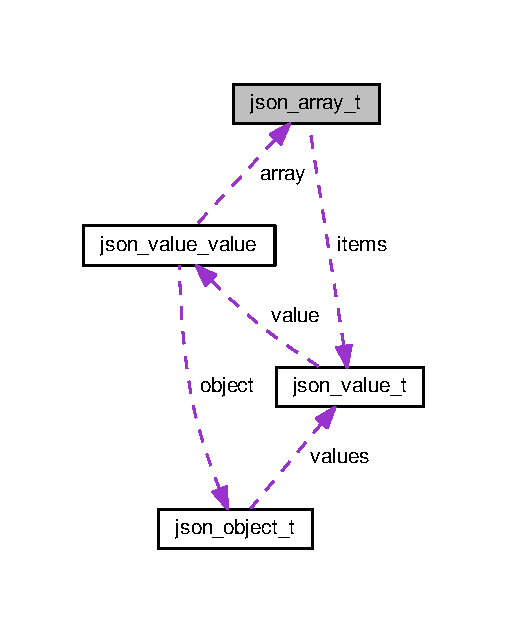
\includegraphics[width=243pt]{structjson__array__t__coll__graph}
\end{center}
\end{figure}
\subsection*{Data Fields}
\begin{DoxyCompactItemize}
\item 
\hypertarget{structjson__array__t_a6834c444c0eb10e41117803475c52e12}{\hyperlink{structjson__value__t}{J\-S\-O\-N\-\_\-\-Value} $\ast$$\ast$ {\bfseries items}}\label{structjson__array__t_a6834c444c0eb10e41117803475c52e12}

\item 
\hypertarget{structjson__array__t_a76d971a3c552bc58ba9f0d5fceae9806}{size\-\_\-t {\bfseries count}}\label{structjson__array__t_a76d971a3c552bc58ba9f0d5fceae9806}

\item 
\hypertarget{structjson__array__t_ad721fc6ca6a3d6ba3bc506576622aab0}{size\-\_\-t {\bfseries capacity}}\label{structjson__array__t_ad721fc6ca6a3d6ba3bc506576622aab0}

\end{DoxyCompactItemize}


The documentation for this struct was generated from the following file\-:\begin{DoxyCompactItemize}
\item 
parson/parson.\-c\end{DoxyCompactItemize}

\hypertarget{structjson__object__t}{\section{json\-\_\-object\-\_\-t Struct Reference}
\label{structjson__object__t}\index{json\-\_\-object\-\_\-t@{json\-\_\-object\-\_\-t}}
}


Collaboration diagram for json\-\_\-object\-\_\-t\-:\nopagebreak
\begin{figure}[H]
\begin{center}
\leavevmode
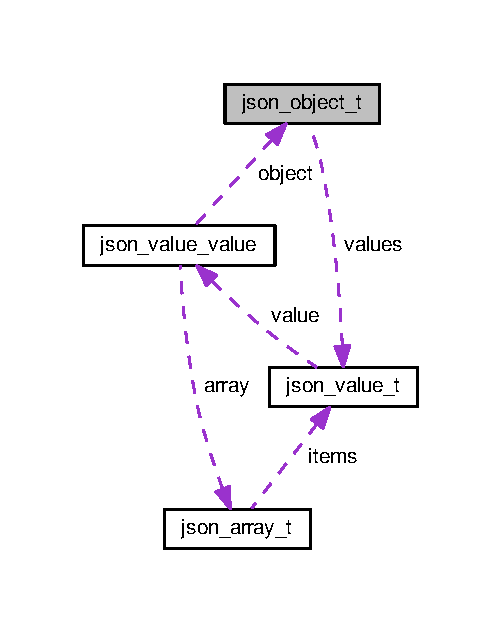
\includegraphics[width=240pt]{structjson__object__t__coll__graph}
\end{center}
\end{figure}
\subsection*{Data Fields}
\begin{DoxyCompactItemize}
\item 
\hypertarget{structjson__object__t_a26fc633cf551a2621e172633486c85ef}{char $\ast$$\ast$ {\bfseries names}}\label{structjson__object__t_a26fc633cf551a2621e172633486c85ef}

\item 
\hypertarget{structjson__object__t_a39e2a988b9b2caaf33034e245a7ee8c0}{\hyperlink{structjson__value__t}{J\-S\-O\-N\-\_\-\-Value} $\ast$$\ast$ {\bfseries values}}\label{structjson__object__t_a39e2a988b9b2caaf33034e245a7ee8c0}

\item 
\hypertarget{structjson__object__t_a76d971a3c552bc58ba9f0d5fceae9806}{size\-\_\-t {\bfseries count}}\label{structjson__object__t_a76d971a3c552bc58ba9f0d5fceae9806}

\item 
\hypertarget{structjson__object__t_ad721fc6ca6a3d6ba3bc506576622aab0}{size\-\_\-t {\bfseries capacity}}\label{structjson__object__t_ad721fc6ca6a3d6ba3bc506576622aab0}

\end{DoxyCompactItemize}


The documentation for this struct was generated from the following file\-:\begin{DoxyCompactItemize}
\item 
parson/parson.\-c\end{DoxyCompactItemize}

\hypertarget{structjson__value__t}{\section{json\-\_\-value\-\_\-t Struct Reference}
\label{structjson__value__t}\index{json\-\_\-value\-\_\-t@{json\-\_\-value\-\_\-t}}
}


Collaboration diagram for json\-\_\-value\-\_\-t\-:\nopagebreak
\begin{figure}[H]
\begin{center}
\leavevmode
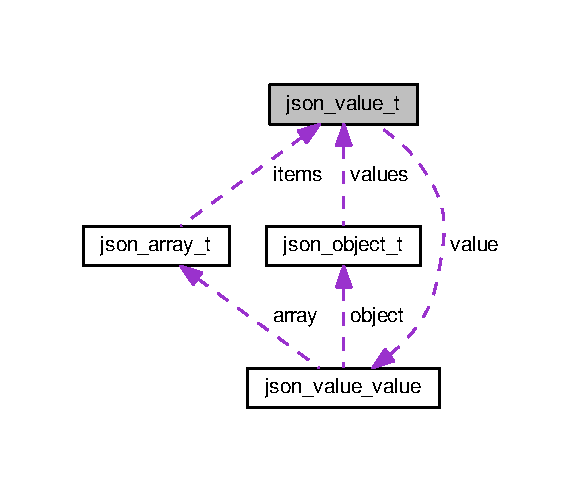
\includegraphics[width=280pt]{structjson__value__t__coll__graph}
\end{center}
\end{figure}
\subsection*{Data Fields}
\begin{DoxyCompactItemize}
\item 
\hypertarget{structjson__value__t_a374a05c01497eb7769eec2ab26cd95b6}{J\-S\-O\-N\-\_\-\-Value\-\_\-\-Type {\bfseries type}}\label{structjson__value__t_a374a05c01497eb7769eec2ab26cd95b6}

\item 
\hypertarget{structjson__value__t_a96135d87b37e477357e5d43811aaa3f1}{\hyperlink{unionjson__value__value}{J\-S\-O\-N\-\_\-\-Value\-\_\-\-Value} {\bfseries value}}\label{structjson__value__t_a96135d87b37e477357e5d43811aaa3f1}

\end{DoxyCompactItemize}


The documentation for this struct was generated from the following file\-:\begin{DoxyCompactItemize}
\item 
parson/parson.\-c\end{DoxyCompactItemize}

\hypertarget{unionjson__value__value}{\section{json\-\_\-value\-\_\-value Union Reference}
\label{unionjson__value__value}\index{json\-\_\-value\-\_\-value@{json\-\_\-value\-\_\-value}}
}


Collaboration diagram for json\-\_\-value\-\_\-value\-:\nopagebreak
\begin{figure}[H]
\begin{center}
\leavevmode
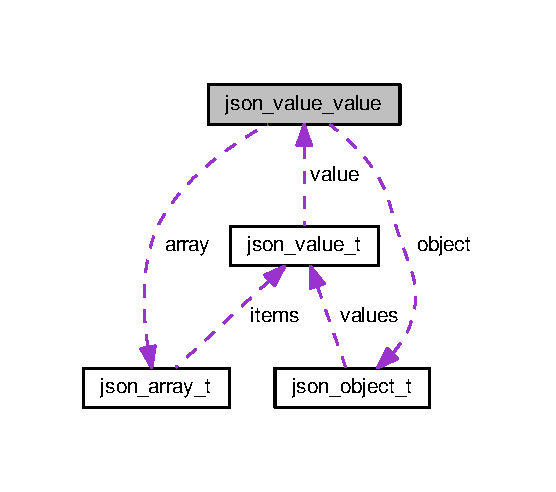
\includegraphics[width=267pt]{unionjson__value__value__coll__graph}
\end{center}
\end{figure}
\subsection*{Data Fields}
\begin{DoxyCompactItemize}
\item 
\hypertarget{unionjson__value__value_aed1cfb225a5fb77461e7972691e68a72}{char $\ast$ {\bfseries string}}\label{unionjson__value__value_aed1cfb225a5fb77461e7972691e68a72}

\item 
\hypertarget{unionjson__value__value_a01b4671c6b7cc8f831c951c000a37735}{double {\bfseries number}}\label{unionjson__value__value_a01b4671c6b7cc8f831c951c000a37735}

\item 
\hypertarget{unionjson__value__value_adf328f722d277e72d53cb9ba3dc24b89}{\hyperlink{structjson__object__t}{J\-S\-O\-N\-\_\-\-Object} $\ast$ {\bfseries object}}\label{unionjson__value__value_adf328f722d277e72d53cb9ba3dc24b89}

\item 
\hypertarget{unionjson__value__value_a22a00745be0ac60b4123d170b7197c7b}{\hyperlink{structjson__array__t}{J\-S\-O\-N\-\_\-\-Array} $\ast$ {\bfseries array}}\label{unionjson__value__value_a22a00745be0ac60b4123d170b7197c7b}

\item 
\hypertarget{unionjson__value__value_afc58e0c0df35925913174accbf1114cb}{int {\bfseries boolean}}\label{unionjson__value__value_afc58e0c0df35925913174accbf1114cb}

\item 
\hypertarget{unionjson__value__value_a76be38e21d5d7e1dc6da841571762c4d}{int {\bfseries null}}\label{unionjson__value__value_a76be38e21d5d7e1dc6da841571762c4d}

\end{DoxyCompactItemize}


The documentation for this union was generated from the following file\-:\begin{DoxyCompactItemize}
\item 
parson/parson.\-c\end{DoxyCompactItemize}

\hypertarget{structpull__resp}{\section{pull\-\_\-resp Struct Reference}
\label{structpull__resp}\index{pull\-\_\-resp@{pull\-\_\-resp}}
}
\subsection*{Data Fields}
\begin{DoxyCompactItemize}
\item 
\hypertarget{structpull__resp_a02849de4c9014b33209233e7111f732b}{byte {\bfseries protocol}}\label{structpull__resp_a02849de4c9014b33209233e7111f732b}

\item 
\hypertarget{structpull__resp_ae7dfa7db7be91bb9fdaa8d3497a50ce7}{byte {\bfseries unused} \mbox{[}2\mbox{]}}\label{structpull__resp_ae7dfa7db7be91bb9fdaa8d3497a50ce7}

\item 
\hypertarget{structpull__resp_ac9af2606678b0b985667c0b97b5ef8b5}{byte {\bfseries id}}\label{structpull__resp_ac9af2606678b0b985667c0b97b5ef8b5}

\item 
\hypertarget{structpull__resp_ae75ec805c7e74dcf4dae969c03d32661}{char {\bfseries data} \mbox{[}2048\mbox{]}}\label{structpull__resp_ae75ec805c7e74dcf4dae969c03d32661}

\end{DoxyCompactItemize}


\subsection{Detailed Description}
\paragraph*{5.\-4. P\-U\-L\-L\-\_\-\-R\-E\-S\-P packet}

That packet type is used by the server to send R\-F packets and associated metadata that will have to be emitted by the gateway.

\begin{TabularC}{2}
\hline
\rowcolor{lightgray}\PBS\centering {\bf Bytes }&{\bf Function  }\\\cline{1-2}
\PBS\centering 0 &protocol version = 1 \\\cline{1-2}
\PBS\centering 1-\/2 &unused bytes \\\cline{1-2}
\PBS\centering 3 &P\-U\-L\-L\-\_\-\-R\-E\-S\-P identifier 0x03 \\\cline{1-2}
\PBS\centering 4-\/end &J\-S\-O\-N object, starting with \{, ending with \}, see section 6 \\\cline{1-2}
\end{TabularC}


\begin{TabularC}{3}
\hline
\rowcolor{lightgray}\PBS\centering {\bf Name }&\PBS\centering {\bf Type }&{\bf Function  }\\\cline{1-3}
\PBS\centering imme &\PBS\centering bool &Send packet immediately (will ignore tmst \& time) \\\cline{1-3}
\PBS\centering tmst &\PBS\centering number &Send packet on a certain timestamp value (will ignore time) \\\cline{1-3}
\PBS\centering time &\PBS\centering string &Send packet at a certain time (G\-P\-S synchronization required) \\\cline{1-3}
\PBS\centering freq &\PBS\centering number &T\-X central frequency in M\-Hz (unsigned float, Hz precision) \\\cline{1-3}
\PBS\centering rfch &\PBS\centering number &Concentrator \char`\"{}\-R\-F chain\char`\"{} used for T\-X (unsigned integer) \\\cline{1-3}
\PBS\centering powe &\PBS\centering number &T\-X output power in d\-Bm (unsigned integer, d\-Bm precision) \\\cline{1-3}
\PBS\centering modu &\PBS\centering string &Modulation identifier \char`\"{}\-L\-O\-R\-A\char`\"{} or \char`\"{}\-F\-S\-K\char`\"{} \\\cline{1-3}
\PBS\centering datr &\PBS\centering string &Lo\-Ra datarate identifier (eg. S\-F12\-B\-W500) \\\cline{1-3}
\PBS\centering datr &\PBS\centering number &F\-S\-K datarate (unsigned, in bits per second) \\\cline{1-3}
\PBS\centering codr &\PBS\centering string &Lo\-Ra E\-C\-C coding rate identifier \\\cline{1-3}
\PBS\centering fdev &\PBS\centering number &F\-S\-K frequency deviation (unsigned integer, in Hz) \\\cline{1-3}
\PBS\centering ipol &\PBS\centering bool &Lora modulation polarization inversion \\\cline{1-3}
\PBS\centering prea &\PBS\centering number &R\-F preamble size (unsigned integer) \\\cline{1-3}
\PBS\centering size &\PBS\centering number &R\-F packet payload size in bytes (unsigned integer) \\\cline{1-3}
\PBS\centering data &\PBS\centering string &Base64 encoded R\-F packet payload, padding optional \\\cline{1-3}
\PBS\centering ncrc &\PBS\centering bool &If true, disable the C\-R\-C of the physical layer (optional) \\\cline{1-3}
\end{TabularC}


The documentation for this struct was generated from the following file\-:\begin{DoxyCompactItemize}
\item 
src/send\-\_\-downstream\-\_\-message.\-c\end{DoxyCompactItemize}

\hypertarget{structrxpk}{\section{rxpk Struct Reference}
\label{structrxpk}\index{rxpk@{rxpk}}
}


Collaboration diagram for rxpk\-:\nopagebreak
\begin{figure}[H]
\begin{center}
\leavevmode
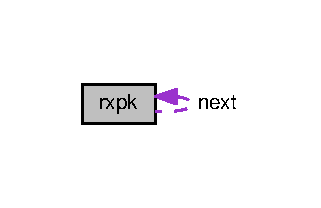
\includegraphics[width=154pt]{structrxpk__coll__graph}
\end{center}
\end{figure}
\subsection*{Data Fields}
\begin{DoxyCompactItemize}
\item 
\hypertarget{structrxpk_a7ba42be95635137cb867f08c8aa01f3b}{char {\bfseries time} \mbox{[}35\mbox{]}}\label{structrxpk_a7ba42be95635137cb867f08c8aa01f3b}

\item 
\hypertarget{structrxpk_a84a0544333ed45665260e3971494c96c}{uint32\-\_\-t {\bfseries tmst}}\label{structrxpk_a84a0544333ed45665260e3971494c96c}

\item 
\hypertarget{structrxpk_a26aea75a25190af8d4bebf654888935d}{double {\bfseries freq}}\label{structrxpk_a26aea75a25190af8d4bebf654888935d}

\item 
\hypertarget{structrxpk_a9f2a059618fb285e162d95b79991efa7}{unsigned int {\bfseries channel}}\label{structrxpk_a9f2a059618fb285e162d95b79991efa7}

\item 
\hypertarget{structrxpk_a566a9646361d592aa0be3fe468b29aad}{unsigned int {\bfseries rf\-\_\-channel}}\label{structrxpk_a566a9646361d592aa0be3fe468b29aad}

\item 
\hypertarget{structrxpk_a7d6f8a25e94209bd3ba29b2051ca4f08}{int {\bfseries stat}\-:1}\label{structrxpk_a7d6f8a25e94209bd3ba29b2051ca4f08}

\item 
\hypertarget{structrxpk_a167264916b5fad13dd3dc470128e3eef}{char {\bfseries modulation} \mbox{[}5\mbox{]}}\label{structrxpk_a167264916b5fad13dd3dc470128e3eef}

\item 
\hypertarget{structrxpk_a96f84d084cdf0e910c2482be0632fa97}{char {\bfseries datarate} \mbox{[}15\mbox{]}}\label{structrxpk_a96f84d084cdf0e910c2482be0632fa97}

\item 
\hypertarget{structrxpk_ae4bd55e8e15052cb4ac21a9aba5866ad}{unsigned int {\bfseries fsk\-\_\-datarate}}\label{structrxpk_ae4bd55e8e15052cb4ac21a9aba5866ad}

\item 
\hypertarget{structrxpk_acff1848d3803c5bb5a4afdee8b73e17a}{char {\bfseries coding\-\_\-rate} \mbox{[}10\mbox{]}}\label{structrxpk_acff1848d3803c5bb5a4afdee8b73e17a}

\item 
\hypertarget{structrxpk_ab6f4522a5a5c4577c16d0e23339a1414}{int {\bfseries rssi}}\label{structrxpk_ab6f4522a5a5c4577c16d0e23339a1414}

\item 
\hypertarget{structrxpk_a31a715ebcd5579924b4d67ca9009e7e6}{double {\bfseries snr}}\label{structrxpk_a31a715ebcd5579924b4d67ca9009e7e6}

\item 
\hypertarget{structrxpk_aee1a30bf4a12e49db87ac9751f93549b}{unsigned int {\bfseries packet\-\_\-size}}\label{structrxpk_aee1a30bf4a12e49db87ac9751f93549b}

\item 
\hypertarget{structrxpk_a18f141cb2726073503afb9f1d6c85efb}{char $\ast$ {\bfseries payload}}\label{structrxpk_a18f141cb2726073503afb9f1d6c85efb}

\item 
\hypertarget{structrxpk_a5455ebea0dde09f27d432e404a4d9f71}{struct \hyperlink{structrxpk}{rxpk} $\ast$ {\bfseries next}}\label{structrxpk_a5455ebea0dde09f27d432e404a4d9f71}

\end{DoxyCompactItemize}


The documentation for this struct was generated from the following file\-:\begin{DoxyCompactItemize}
\item 
includes/upstream\-\_\-packet.\-h\end{DoxyCompactItemize}

\hypertarget{structupstream__packet}{\section{upstream\-\_\-packet Struct Reference}
\label{structupstream__packet}\index{upstream\-\_\-packet@{upstream\-\_\-packet}}
}


Collaboration diagram for upstream\-\_\-packet\-:\nopagebreak
\begin{figure}[H]
\begin{center}
\leavevmode
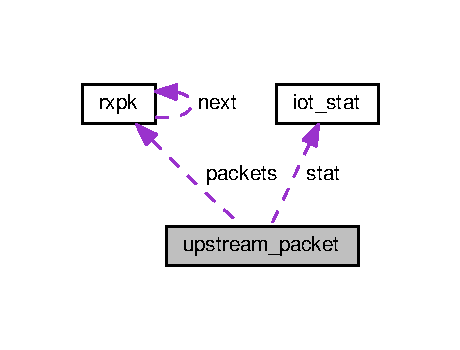
\includegraphics[width=221pt]{structupstream__packet__coll__graph}
\end{center}
\end{figure}
\subsection*{Data Fields}
\begin{DoxyCompactItemize}
\item 
\hypertarget{structupstream__packet_abe86b4951b6df6fbb6d7bbf7d014f125}{\hyperlink{structiot__stat}{iot\-\_\-stat} {\bfseries stat}}\label{structupstream__packet_abe86b4951b6df6fbb6d7bbf7d014f125}

\item 
\hypertarget{structupstream__packet_a4ed16bb642cf466d4d284c9f46bc0805}{\hyperlink{structrxpk}{rxpk} $\ast$ {\bfseries packets}}\label{structupstream__packet_a4ed16bb642cf466d4d284c9f46bc0805}

\end{DoxyCompactItemize}


The documentation for this struct was generated from the following file\-:\begin{DoxyCompactItemize}
\item 
includes/upstream\-\_\-packet.\-h\end{DoxyCompactItemize}

\chapter{File Documentation}
\hypertarget{constants_8h}{\section{includes/constants.h File Reference}
\label{constants_8h}\index{includes/constants.\-h@{includes/constants.\-h}}
}


This file defines some constants used in the program.  


This graph shows which files directly or indirectly include this file\-:\nopagebreak
\begin{figure}[H]
\begin{center}
\leavevmode
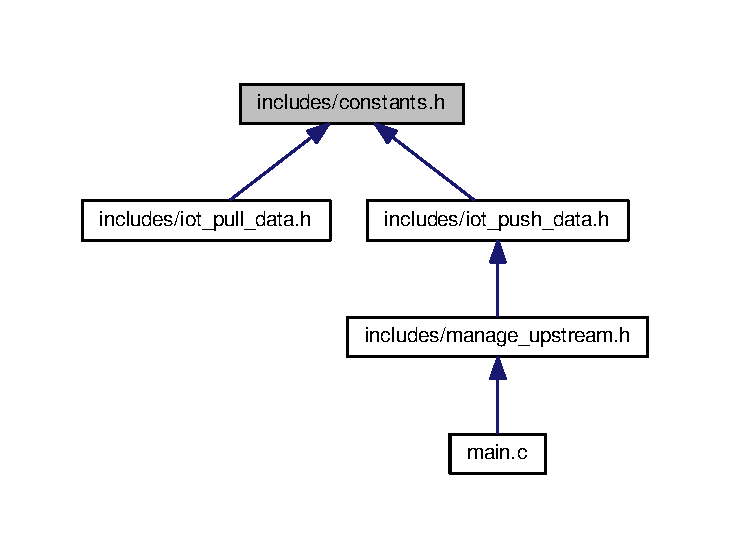
\includegraphics[width=350pt]{constants_8h__dep__incl}
\end{center}
\end{figure}
\subsection*{Macros}
\begin{DoxyCompactItemize}
\item 
\#define \hyperlink{constants_8h_a3a7ac43414dac22430805b0fd94d3484}{M\-A\-X\-\_\-\-U\-P\-S\-T\-R\-E\-A\-M\-\_\-\-E\-R\-R\-O\-R}~5
\item 
\#define \hyperlink{constants_8h_a2db560f9b69224481e55114e1007fb9f}{M\-A\-X\-\_\-\-D\-O\-W\-N\-S\-T\-R\-E\-A\-M\-\_\-\-E\-R\-R\-O\-R}~5
\item 
\#define \hyperlink{constants_8h_a786442238545011e2a0eb7ce468ad692}{I\-N\-C\-O\-M\-M\-I\-N\-G\-\_\-\-M\-S\-G\-\_\-\-S\-I\-Z\-E}~2048
\item 
\#define \hyperlink{constants_8h_a26769957ec1a2beaf223f33b66ee64ab}{I\-N\-V\-A\-L\-I\-D\-\_\-\-S\-O\-C\-K\-E\-T}~-\/1
\item 
\#define \hyperlink{constants_8h_a633b0396ff93d336a088412a190a5072}{S\-O\-C\-K\-E\-T\-\_\-\-E\-R\-R\-O\-R}~-\/2
\item 
\#define \hyperlink{constants_8h_a3ea8fe7de431e387d4538385fa582893}{J\-S\-O\-N\-\_\-\-B\-A\-D\-\_\-\-F\-O\-R\-M\-E\-D}~-\/3
\end{DoxyCompactItemize}


\subsection{Detailed Description}
This file defines some constants used in the program. \begin{DoxyAuthor}{Author}
Giuliano Franchetto 
\end{DoxyAuthor}
\begin{DoxyDate}{Date}
30/09/2015 
\end{DoxyDate}
\begin{DoxyVersion}{Version}
1 
\end{DoxyVersion}


\subsection{Macro Definition Documentation}
\hypertarget{constants_8h_a786442238545011e2a0eb7ce468ad692}{\index{constants.\-h@{constants.\-h}!I\-N\-C\-O\-M\-M\-I\-N\-G\-\_\-\-M\-S\-G\-\_\-\-S\-I\-Z\-E@{I\-N\-C\-O\-M\-M\-I\-N\-G\-\_\-\-M\-S\-G\-\_\-\-S\-I\-Z\-E}}
\index{I\-N\-C\-O\-M\-M\-I\-N\-G\-\_\-\-M\-S\-G\-\_\-\-S\-I\-Z\-E@{I\-N\-C\-O\-M\-M\-I\-N\-G\-\_\-\-M\-S\-G\-\_\-\-S\-I\-Z\-E}!constants.h@{constants.\-h}}
\subsubsection[{I\-N\-C\-O\-M\-M\-I\-N\-G\-\_\-\-M\-S\-G\-\_\-\-S\-I\-Z\-E}]{\setlength{\rightskip}{0pt plus 5cm}\#define I\-N\-C\-O\-M\-M\-I\-N\-G\-\_\-\-M\-S\-G\-\_\-\-S\-I\-Z\-E~2048}}\label{constants_8h_a786442238545011e2a0eb7ce468ad692}
This is the maximum size of a packet sent by the Io\-T station to the program. This is not robust, but for the first version, this will do it \hypertarget{constants_8h_a26769957ec1a2beaf223f33b66ee64ab}{\index{constants.\-h@{constants.\-h}!I\-N\-V\-A\-L\-I\-D\-\_\-\-S\-O\-C\-K\-E\-T@{I\-N\-V\-A\-L\-I\-D\-\_\-\-S\-O\-C\-K\-E\-T}}
\index{I\-N\-V\-A\-L\-I\-D\-\_\-\-S\-O\-C\-K\-E\-T@{I\-N\-V\-A\-L\-I\-D\-\_\-\-S\-O\-C\-K\-E\-T}!constants.h@{constants.\-h}}
\subsubsection[{I\-N\-V\-A\-L\-I\-D\-\_\-\-S\-O\-C\-K\-E\-T}]{\setlength{\rightskip}{0pt plus 5cm}\#define I\-N\-V\-A\-L\-I\-D\-\_\-\-S\-O\-C\-K\-E\-T~-\/1}}\label{constants_8h_a26769957ec1a2beaf223f33b66ee64ab}
Error code returned when creating a socket fails \hypertarget{constants_8h_a3ea8fe7de431e387d4538385fa582893}{\index{constants.\-h@{constants.\-h}!J\-S\-O\-N\-\_\-\-B\-A\-D\-\_\-\-F\-O\-R\-M\-E\-D@{J\-S\-O\-N\-\_\-\-B\-A\-D\-\_\-\-F\-O\-R\-M\-E\-D}}
\index{J\-S\-O\-N\-\_\-\-B\-A\-D\-\_\-\-F\-O\-R\-M\-E\-D@{J\-S\-O\-N\-\_\-\-B\-A\-D\-\_\-\-F\-O\-R\-M\-E\-D}!constants.h@{constants.\-h}}
\subsubsection[{J\-S\-O\-N\-\_\-\-B\-A\-D\-\_\-\-F\-O\-R\-M\-E\-D}]{\setlength{\rightskip}{0pt plus 5cm}\#define J\-S\-O\-N\-\_\-\-B\-A\-D\-\_\-\-F\-O\-R\-M\-E\-D~-\/3}}\label{constants_8h_a3ea8fe7de431e387d4538385fa582893}
Error code returned when a J\-S\-O\-N sent by the Io\-T station is malformed \hypertarget{constants_8h_a2db560f9b69224481e55114e1007fb9f}{\index{constants.\-h@{constants.\-h}!M\-A\-X\-\_\-\-D\-O\-W\-N\-S\-T\-R\-E\-A\-M\-\_\-\-E\-R\-R\-O\-R@{M\-A\-X\-\_\-\-D\-O\-W\-N\-S\-T\-R\-E\-A\-M\-\_\-\-E\-R\-R\-O\-R}}
\index{M\-A\-X\-\_\-\-D\-O\-W\-N\-S\-T\-R\-E\-A\-M\-\_\-\-E\-R\-R\-O\-R@{M\-A\-X\-\_\-\-D\-O\-W\-N\-S\-T\-R\-E\-A\-M\-\_\-\-E\-R\-R\-O\-R}!constants.h@{constants.\-h}}
\subsubsection[{M\-A\-X\-\_\-\-D\-O\-W\-N\-S\-T\-R\-E\-A\-M\-\_\-\-E\-R\-R\-O\-R}]{\setlength{\rightskip}{0pt plus 5cm}\#define M\-A\-X\-\_\-\-D\-O\-W\-N\-S\-T\-R\-E\-A\-M\-\_\-\-E\-R\-R\-O\-R~5}}\label{constants_8h_a2db560f9b69224481e55114e1007fb9f}
This field defines the number of allowed error before closing the downstream socket with the Io\-T station \hypertarget{constants_8h_a3a7ac43414dac22430805b0fd94d3484}{\index{constants.\-h@{constants.\-h}!M\-A\-X\-\_\-\-U\-P\-S\-T\-R\-E\-A\-M\-\_\-\-E\-R\-R\-O\-R@{M\-A\-X\-\_\-\-U\-P\-S\-T\-R\-E\-A\-M\-\_\-\-E\-R\-R\-O\-R}}
\index{M\-A\-X\-\_\-\-U\-P\-S\-T\-R\-E\-A\-M\-\_\-\-E\-R\-R\-O\-R@{M\-A\-X\-\_\-\-U\-P\-S\-T\-R\-E\-A\-M\-\_\-\-E\-R\-R\-O\-R}!constants.h@{constants.\-h}}
\subsubsection[{M\-A\-X\-\_\-\-U\-P\-S\-T\-R\-E\-A\-M\-\_\-\-E\-R\-R\-O\-R}]{\setlength{\rightskip}{0pt plus 5cm}\#define M\-A\-X\-\_\-\-U\-P\-S\-T\-R\-E\-A\-M\-\_\-\-E\-R\-R\-O\-R~5}}\label{constants_8h_a3a7ac43414dac22430805b0fd94d3484}
This field defines the number of allowed error before closing the upstream socket with the Io\-T station \hypertarget{constants_8h_a633b0396ff93d336a088412a190a5072}{\index{constants.\-h@{constants.\-h}!S\-O\-C\-K\-E\-T\-\_\-\-E\-R\-R\-O\-R@{S\-O\-C\-K\-E\-T\-\_\-\-E\-R\-R\-O\-R}}
\index{S\-O\-C\-K\-E\-T\-\_\-\-E\-R\-R\-O\-R@{S\-O\-C\-K\-E\-T\-\_\-\-E\-R\-R\-O\-R}!constants.h@{constants.\-h}}
\subsubsection[{S\-O\-C\-K\-E\-T\-\_\-\-E\-R\-R\-O\-R}]{\setlength{\rightskip}{0pt plus 5cm}\#define S\-O\-C\-K\-E\-T\-\_\-\-E\-R\-R\-O\-R~-\/2}}\label{constants_8h_a633b0396ff93d336a088412a190a5072}
Error code returned when a read/write operation fails 
\hypertarget{downstream__packet_8h}{\section{includes/downstream\-\_\-packet.h File Reference}
\label{downstream__packet_8h}\index{includes/downstream\-\_\-packet.\-h@{includes/downstream\-\_\-packet.\-h}}
}


This file defines the structure \char`\"{}downstream\-\_\-packet\char`\"{}.  


{\ttfamily \#include $<$stdbool.\-h$>$}\\*
Include dependency graph for downstream\-\_\-packet.\-h\-:\nopagebreak
\begin{figure}[H]
\begin{center}
\leavevmode
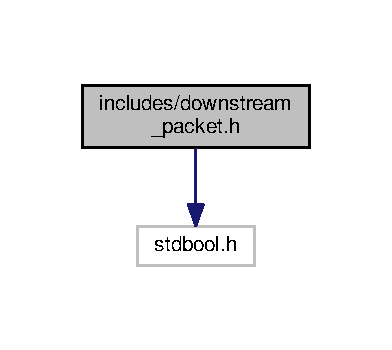
\includegraphics[width=188pt]{downstream__packet_8h__incl}
\end{center}
\end{figure}
This graph shows which files directly or indirectly include this file\-:\nopagebreak
\begin{figure}[H]
\begin{center}
\leavevmode
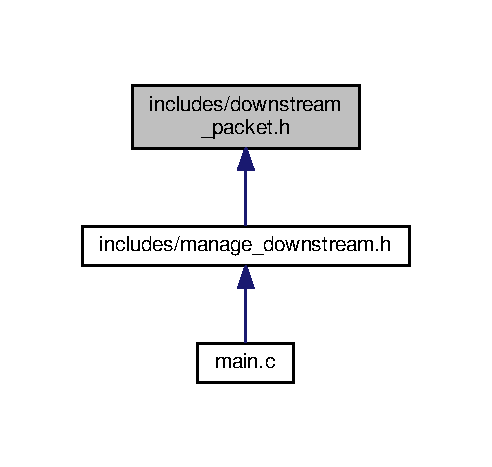
\includegraphics[width=236pt]{downstream__packet_8h__dep__incl}
\end{center}
\end{figure}
\subsection*{Data Structures}
\begin{DoxyCompactItemize}
\item 
struct \hyperlink{structdownstream__packet}{downstream\-\_\-packet}
\begin{DoxyCompactList}\small\item\em This structure represents a package that must be sent to the Io\-T station to make it send a Lo\-Ra message Some of these fields are optional. \end{DoxyCompactList}\end{DoxyCompactItemize}


\subsection{Detailed Description}
This file defines the structure \char`\"{}downstream\-\_\-packet\char`\"{}. \begin{DoxyAuthor}{Author}
Giuliano Franchetto 
\end{DoxyAuthor}
\begin{DoxyDate}{Date}
30/09/2015 
\end{DoxyDate}
\begin{DoxyVersion}{Version}
1
\end{DoxyVersion}
The reader can find the official documentation on this url\-: \href{https://github.com/Lora-net/packet_forwarder/blob/master/PROTOCOL.TXT}{\tt https\-://github.\-com/\-Lora-\/net/packet\-\_\-forwarder/blob/master/\-P\-R\-O\-T\-O\-C\-O\-L.\-T\-X\-T} 
\hypertarget{iot__pull__data_8h}{\section{includes/iot\-\_\-pull\-\_\-data.h File Reference}
\label{iot__pull__data_8h}\index{includes/iot\-\_\-pull\-\_\-data.\-h@{includes/iot\-\_\-pull\-\_\-data.\-h}}
}


This file defines a structure used to represent the pull\-\_\-data message sent by the Io\-T station.  


{\ttfamily \#include $<$constants.\-h$>$}\\*
{\ttfamily \#include $<$types.\-h$>$}\\*
Include dependency graph for iot\-\_\-pull\-\_\-data.\-h\-:\nopagebreak
\begin{figure}[H]
\begin{center}
\leavevmode
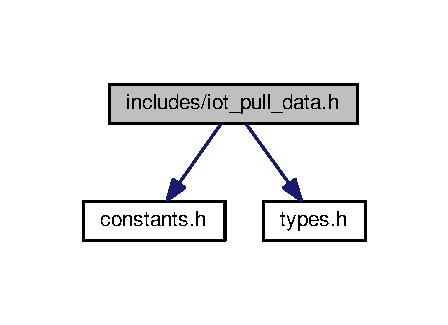
\includegraphics[width=215pt]{iot__pull__data_8h__incl}
\end{center}
\end{figure}
\subsection*{Data Structures}
\begin{DoxyCompactItemize}
\item 
union \hyperlink{unioniot__pull__data}{iot\-\_\-pull\-\_\-data}
\end{DoxyCompactItemize}


\subsection{Detailed Description}
This file defines a structure used to represent the pull\-\_\-data message sent by the Io\-T station. \begin{DoxyAuthor}{Author}
Giuliano Franchetto 
\end{DoxyAuthor}
\begin{DoxyDate}{Date}
30/09/2015 
\end{DoxyDate}
\begin{DoxyVersion}{Version}
1 
\end{DoxyVersion}

\hypertarget{iot__push__data_8h}{\section{includes/iot\-\_\-push\-\_\-data.h File Reference}
\label{iot__push__data_8h}\index{includes/iot\-\_\-push\-\_\-data.\-h@{includes/iot\-\_\-push\-\_\-data.\-h}}
}


This file defines a structure used to represent the push\-\_\-data message sent by the Io\-T station.  


{\ttfamily \#include $<$constants.\-h$>$}\\*
{\ttfamily \#include $<$types.\-h$>$}\\*
Include dependency graph for iot\-\_\-push\-\_\-data.\-h\-:\nopagebreak
\begin{figure}[H]
\begin{center}
\leavevmode
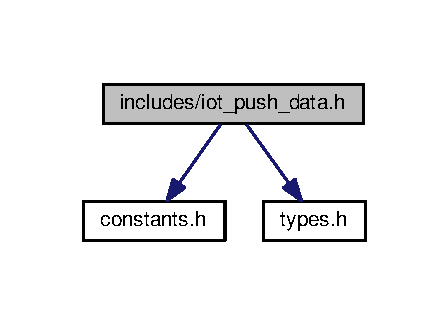
\includegraphics[width=215pt]{iot__push__data_8h__incl}
\end{center}
\end{figure}
This graph shows which files directly or indirectly include this file\-:\nopagebreak
\begin{figure}[H]
\begin{center}
\leavevmode
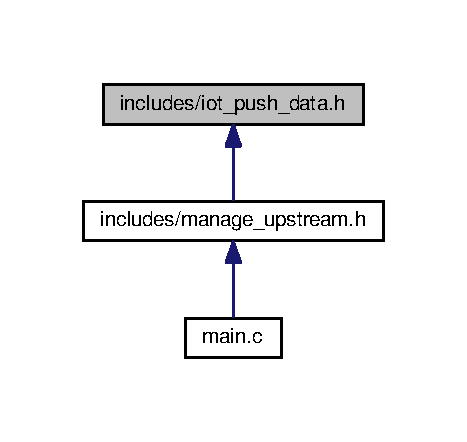
\includegraphics[width=224pt]{iot__push__data_8h__dep__incl}
\end{center}
\end{figure}
\subsection*{Data Structures}
\begin{DoxyCompactItemize}
\item 
union \hyperlink{unioniot__push__data}{iot\-\_\-push\-\_\-data}
\begin{DoxyCompactList}\small\item\em To have more information about this structure, look at the \hyperlink{unioniot__pull__data}{iot\-\_\-pull\-\_\-data}. \end{DoxyCompactList}\end{DoxyCompactItemize}


\subsection{Detailed Description}
This file defines a structure used to represent the push\-\_\-data message sent by the Io\-T station. \begin{DoxyAuthor}{Author}
Giuliano Franchetto 
\end{DoxyAuthor}
\begin{DoxyDate}{Date}
30/09/2015 
\end{DoxyDate}
\begin{DoxyVersion}{Version}
1 
\end{DoxyVersion}

\hypertarget{manage__downstream_8h}{\section{includes/manage\-\_\-downstream.h File Reference}
\label{manage__downstream_8h}\index{includes/manage\-\_\-downstream.\-h@{includes/manage\-\_\-downstream.\-h}}
}


This file defines some function prototypes and global variables.  


{\ttfamily \#include $<$stdbool.\-h$>$}\\*
{\ttfamily \#include $<$downstream\-\_\-packet.\-h$>$}\\*
{\ttfamily \#include $<$pthread.\-h$>$}\\*
{\ttfamily \#include $<$netinet/in.\-h$>$}\\*
Include dependency graph for manage\-\_\-downstream.\-h\-:\nopagebreak
\begin{figure}[H]
\begin{center}
\leavevmode
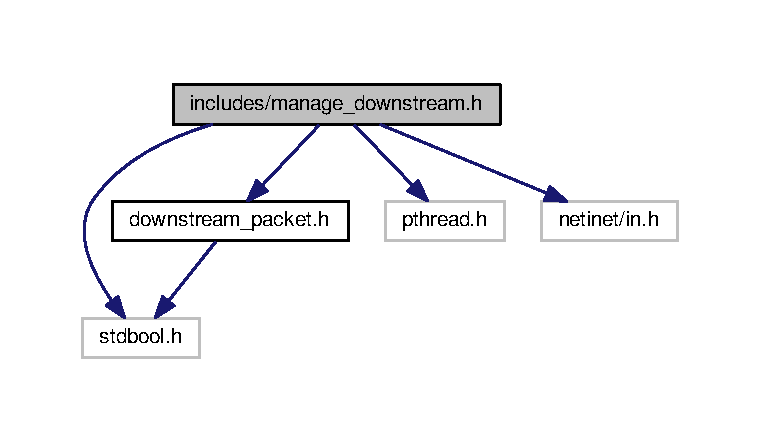
\includegraphics[width=350pt]{manage__downstream_8h__incl}
\end{center}
\end{figure}
This graph shows which files directly or indirectly include this file\-:\nopagebreak
\begin{figure}[H]
\begin{center}
\leavevmode
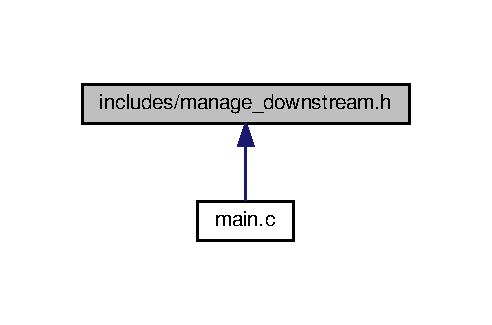
\includegraphics[width=236pt]{manage__downstream_8h__dep__incl}
\end{center}
\end{figure}
\subsection*{Functions}
\begin{DoxyCompactItemize}
\item 
int \hyperlink{manage__downstream_8h_a239658676acc5572c58ccad11e7214cd}{send\-\_\-downstream\-\_\-message} (S\-O\-C\-K\-E\-T socket, struct sockaddr\-\_\-in from, socklen\-\_\-t size, \hyperlink{structdownstream__packet}{downstream\-\_\-packet} packet, bool use\-\_\-minimum\-\_\-data)
\begin{DoxyCompactList}\small\item\em This function send a message to the Io\-T station. This message will next be sent in Lo\-Ra. \end{DoxyCompactList}\item 
void $\ast$ \hyperlink{manage__downstream_8h_a045bea38624e1935146222398772ab42}{manage\-\_\-downstream} (void $\ast$r)
\begin{DoxyCompactList}\small\item\em The thread routine called by main. \end{DoxyCompactList}\end{DoxyCompactItemize}
\subsection*{Variables}
\begin{DoxyCompactItemize}
\item 
pthread\-\_\-t \hyperlink{manage__downstream_8h_a2a9b27e18263ba28e7bf1dda832cff0e}{thread\-\_\-manage\-\_\-downstream}
\item 
bool \hyperlink{manage__downstream_8h_ad54e3fbaaf4a33c07d9a070bf3986a0a}{stop\-\_\-thread\-\_\-downstream}
\item 
int \hyperlink{manage__downstream_8h_a14c8d3b0c27669fa3961afc367df7a77}{downstream\-\_\-error}
\end{DoxyCompactItemize}


\subsection{Detailed Description}
This file defines some function prototypes and global variables. \begin{DoxyAuthor}{Author}
Giuliano Franchetto 
\end{DoxyAuthor}
\begin{DoxyDate}{Date}
30/09/2015 
\end{DoxyDate}
\begin{DoxyVersion}{Version}
1 
\end{DoxyVersion}


\subsection{Function Documentation}
\hypertarget{manage__downstream_8h_a045bea38624e1935146222398772ab42}{\index{manage\-\_\-downstream.\-h@{manage\-\_\-downstream.\-h}!manage\-\_\-downstream@{manage\-\_\-downstream}}
\index{manage\-\_\-downstream@{manage\-\_\-downstream}!manage_downstream.h@{manage\-\_\-downstream.\-h}}
\subsubsection[{manage\-\_\-downstream}]{\setlength{\rightskip}{0pt plus 5cm}void $\ast$ manage\-\_\-downstream (
\begin{DoxyParamCaption}
\item[{void $\ast$}]{r}
\end{DoxyParamCaption}
)}}\label{manage__downstream_8h_a045bea38624e1935146222398772ab42}


The thread routine called by main. 


\begin{DoxyParams}{Parameters}
{\em r} & unused param \\
\hline
\end{DoxyParams}
\begin{DoxyReturn}{Returns}
N\-U\-L\-L 
\end{DoxyReturn}


Here is the call graph for this function\-:\nopagebreak
\begin{figure}[H]
\begin{center}
\leavevmode
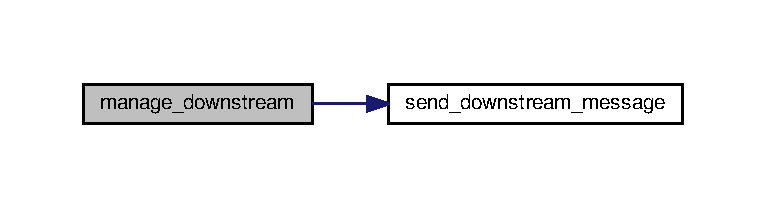
\includegraphics[width=350pt]{manage__downstream_8h_a045bea38624e1935146222398772ab42_cgraph}
\end{center}
\end{figure}


\hypertarget{manage__downstream_8h_a239658676acc5572c58ccad11e7214cd}{\index{manage\-\_\-downstream.\-h@{manage\-\_\-downstream.\-h}!send\-\_\-downstream\-\_\-message@{send\-\_\-downstream\-\_\-message}}
\index{send\-\_\-downstream\-\_\-message@{send\-\_\-downstream\-\_\-message}!manage_downstream.h@{manage\-\_\-downstream.\-h}}
\subsubsection[{send\-\_\-downstream\-\_\-message}]{\setlength{\rightskip}{0pt plus 5cm}int send\-\_\-downstream\-\_\-message (
\begin{DoxyParamCaption}
\item[{S\-O\-C\-K\-E\-T}]{socket, }
\item[{struct sockaddr\-\_\-in}]{from, }
\item[{socklen\-\_\-t}]{size, }
\item[{{\bf downstream\-\_\-packet}}]{packet, }
\item[{bool}]{use\-\_\-minimum\-\_\-data}
\end{DoxyParamCaption}
)}}\label{manage__downstream_8h_a239658676acc5572c58ccad11e7214cd}


This function send a message to the Io\-T station. This message will next be sent in Lo\-Ra. 


\begin{DoxyParams}{Parameters}
{\em socket} & the udp socket with the Io\-T station \\
\hline
{\em from} & a sockaddr\-\_\-in structure which defines the communication with the Io\-T station \\
\hline
{\em size} & \\
\hline
{\em packet} & the packet to send to the Io\-T station, see \hyperlink{structdownstream__packet}{downstream\-\_\-packet} \\
\hline
{\em use\-\_\-minimum\-\_\-data} & packet will be filled with default data in some fields. Needs to be set to true for the moment\\
\hline
\end{DoxyParams}
\begin{DoxyReturn}{Returns}
0 on success, or the errno code 
\end{DoxyReturn}


\subsection{Variable Documentation}
\hypertarget{manage__downstream_8h_a14c8d3b0c27669fa3961afc367df7a77}{\index{manage\-\_\-downstream.\-h@{manage\-\_\-downstream.\-h}!downstream\-\_\-error@{downstream\-\_\-error}}
\index{downstream\-\_\-error@{downstream\-\_\-error}!manage_downstream.h@{manage\-\_\-downstream.\-h}}
\subsubsection[{downstream\-\_\-error}]{\setlength{\rightskip}{0pt plus 5cm}int downstream\-\_\-error}}\label{manage__downstream_8h_a14c8d3b0c27669fa3961afc367df7a77}
The number of error this thread made \hypertarget{manage__downstream_8h_ad54e3fbaaf4a33c07d9a070bf3986a0a}{\index{manage\-\_\-downstream.\-h@{manage\-\_\-downstream.\-h}!stop\-\_\-thread\-\_\-downstream@{stop\-\_\-thread\-\_\-downstream}}
\index{stop\-\_\-thread\-\_\-downstream@{stop\-\_\-thread\-\_\-downstream}!manage_downstream.h@{manage\-\_\-downstream.\-h}}
\subsubsection[{stop\-\_\-thread\-\_\-downstream}]{\setlength{\rightskip}{0pt plus 5cm}bool stop\-\_\-thread\-\_\-downstream}}\label{manage__downstream_8h_ad54e3fbaaf4a33c07d9a070bf3986a0a}
A boolean which must set to true to stop the thread \hypertarget{manage__downstream_8h_a2a9b27e18263ba28e7bf1dda832cff0e}{\index{manage\-\_\-downstream.\-h@{manage\-\_\-downstream.\-h}!thread\-\_\-manage\-\_\-downstream@{thread\-\_\-manage\-\_\-downstream}}
\index{thread\-\_\-manage\-\_\-downstream@{thread\-\_\-manage\-\_\-downstream}!manage_downstream.h@{manage\-\_\-downstream.\-h}}
\subsubsection[{thread\-\_\-manage\-\_\-downstream}]{\setlength{\rightskip}{0pt plus 5cm}pthread\-\_\-t thread\-\_\-manage\-\_\-downstream}}\label{manage__downstream_8h_a2a9b27e18263ba28e7bf1dda832cff0e}
The pthread\-\_\-t used for the manage\-\_\-downstream thread 
\hypertarget{manage__upstream_8h}{\section{includes/manage\-\_\-upstream.h File Reference}
\label{manage__upstream_8h}\index{includes/manage\-\_\-upstream.\-h@{includes/manage\-\_\-upstream.\-h}}
}


This file defines some function prototypes and global variables.  


{\ttfamily \#include $<$pthread.\-h$>$}\\*
{\ttfamily \#include $<$stdbool.\-h$>$}\\*
{\ttfamily \#include $<$iot\-\_\-push\-\_\-data.\-h$>$}\\*
{\ttfamily \#include $<$upstream\-\_\-packet.\-h$>$}\\*
Include dependency graph for manage\-\_\-upstream.\-h\-:\nopagebreak
\begin{figure}[H]
\begin{center}
\leavevmode
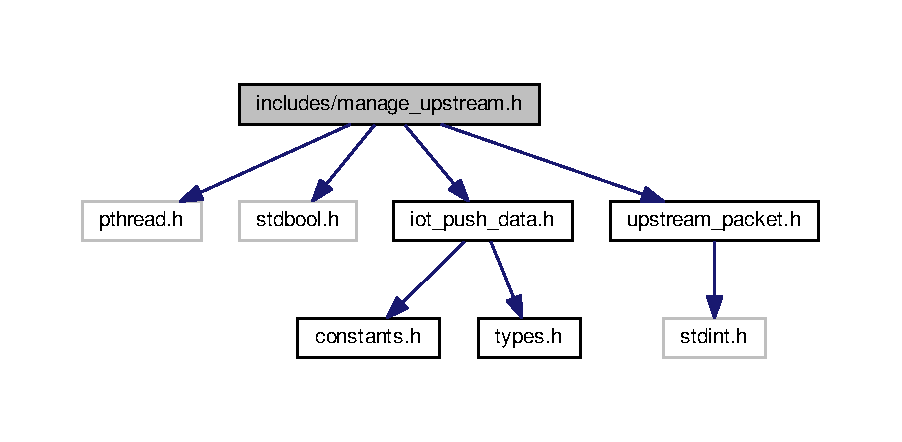
\includegraphics[width=350pt]{manage__upstream_8h__incl}
\end{center}
\end{figure}
This graph shows which files directly or indirectly include this file\-:\nopagebreak
\begin{figure}[H]
\begin{center}
\leavevmode
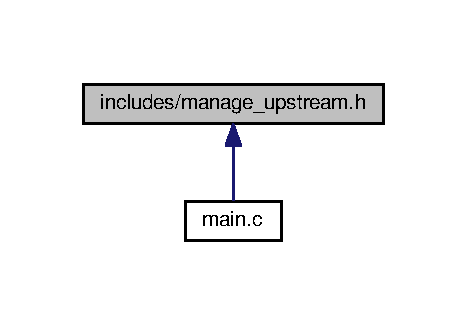
\includegraphics[width=224pt]{manage__upstream_8h__dep__incl}
\end{center}
\end{figure}
\subsection*{Functions}
\begin{DoxyCompactItemize}
\item 
void $\ast$ \hyperlink{manage__upstream_8h_a60c55d3a6d5e77790280275a92a4ba59}{manage\-\_\-upstream} (void $\ast$args)
\begin{DoxyCompactList}\small\item\em The thread routine called by main. \end{DoxyCompactList}\item 
int \hyperlink{manage__upstream_8h_a8ee1dceccf967ddf0d20ad576068c613}{parse\-\_\-upstream\-\_\-json} (\hyperlink{unioniot__push__data}{iot\-\_\-push\-\_\-data} data, \hyperlink{structupstream__packet}{upstream\-\_\-packet} $\ast$packet)
\begin{DoxyCompactList}\small\item\em This function parses a incoming message from the Io\-T station. \end{DoxyCompactList}\item 
void \hyperlink{manage__upstream_8h_a8224dd17e2e125f1f84bb33b7c5ad538}{print\-\_\-upstream\-\_\-packet} (\hyperlink{structupstream__packet}{upstream\-\_\-packet} packet)
\begin{DoxyCompactList}\small\item\em Print a nice message on the console which the data contained in the \hyperlink{structupstream__packet}{upstream\-\_\-packet}. \end{DoxyCompactList}\item 
void \hyperlink{manage__upstream_8h_a81f80bf5317a7b704e747b29414179d3}{free\-\_\-upstream\-\_\-packet} (\hyperlink{structupstream__packet}{upstream\-\_\-packet} $\ast$packet)
\begin{DoxyCompactList}\small\item\em This function frees the linked list in the \hyperlink{structupstream__packet}{upstream\-\_\-packet} packet. \end{DoxyCompactList}\end{DoxyCompactItemize}
\subsection*{Variables}
\begin{DoxyCompactItemize}
\item 
pthread\-\_\-t \hyperlink{manage__upstream_8h_a49e34dce6ea4518b48454896a6ecd171}{thread\-\_\-manage\-\_\-upstream}
\item 
bool \hyperlink{manage__upstream_8h_a4a6f394651f7af3aedb62c255a67bc59}{stop\-\_\-thread\-\_\-upstream}
\item 
int \hyperlink{manage__upstream_8h_a66a09b67a86f445357c6c380f25d1781}{upstream\-\_\-error}
\end{DoxyCompactItemize}


\subsection{Detailed Description}
This file defines some function prototypes and global variables. \begin{DoxyAuthor}{Author}
Giuliano Franchetto 
\end{DoxyAuthor}
\begin{DoxyDate}{Date}
30/09/2015 
\end{DoxyDate}
\begin{DoxyVersion}{Version}
1 
\end{DoxyVersion}


\subsection{Function Documentation}
\hypertarget{manage__upstream_8h_a81f80bf5317a7b704e747b29414179d3}{\index{manage\-\_\-upstream.\-h@{manage\-\_\-upstream.\-h}!free\-\_\-upstream\-\_\-packet@{free\-\_\-upstream\-\_\-packet}}
\index{free\-\_\-upstream\-\_\-packet@{free\-\_\-upstream\-\_\-packet}!manage_upstream.h@{manage\-\_\-upstream.\-h}}
\subsubsection[{free\-\_\-upstream\-\_\-packet}]{\setlength{\rightskip}{0pt plus 5cm}void free\-\_\-upstream\-\_\-packet (
\begin{DoxyParamCaption}
\item[{{\bf upstream\-\_\-packet} $\ast$}]{packet}
\end{DoxyParamCaption}
)}}\label{manage__upstream_8h_a81f80bf5317a7b704e747b29414179d3}


This function frees the linked list in the \hyperlink{structupstream__packet}{upstream\-\_\-packet} packet. 


\begin{DoxyParams}{Parameters}
{\em $\ast$packet} & A pointer to the \hyperlink{structupstream__packet}{upstream\-\_\-packet} to free \\
\hline
\end{DoxyParams}
\begin{DoxyReturn}{Returns}
nothing 
\end{DoxyReturn}
\hypertarget{manage__upstream_8h_a60c55d3a6d5e77790280275a92a4ba59}{\index{manage\-\_\-upstream.\-h@{manage\-\_\-upstream.\-h}!manage\-\_\-upstream@{manage\-\_\-upstream}}
\index{manage\-\_\-upstream@{manage\-\_\-upstream}!manage_upstream.h@{manage\-\_\-upstream.\-h}}
\subsubsection[{manage\-\_\-upstream}]{\setlength{\rightskip}{0pt plus 5cm}void $\ast$ manage\-\_\-upstream (
\begin{DoxyParamCaption}
\item[{void $\ast$}]{r}
\end{DoxyParamCaption}
)}}\label{manage__upstream_8h_a60c55d3a6d5e77790280275a92a4ba59}


The thread routine called by main. 


\begin{DoxyParams}{Parameters}
{\em r} & unused param \\
\hline
\end{DoxyParams}
\begin{DoxyReturn}{Returns}
N\-U\-L\-L 
\end{DoxyReturn}


Here is the call graph for this function\-:\nopagebreak
\begin{figure}[H]
\begin{center}
\leavevmode
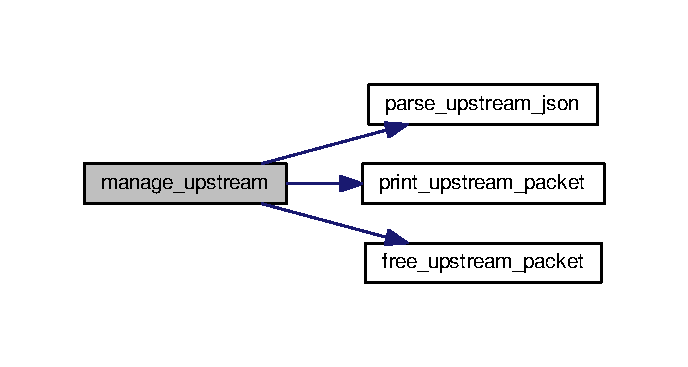
\includegraphics[width=330pt]{manage__upstream_8h_a60c55d3a6d5e77790280275a92a4ba59_cgraph}
\end{center}
\end{figure}


\hypertarget{manage__upstream_8h_a8ee1dceccf967ddf0d20ad576068c613}{\index{manage\-\_\-upstream.\-h@{manage\-\_\-upstream.\-h}!parse\-\_\-upstream\-\_\-json@{parse\-\_\-upstream\-\_\-json}}
\index{parse\-\_\-upstream\-\_\-json@{parse\-\_\-upstream\-\_\-json}!manage_upstream.h@{manage\-\_\-upstream.\-h}}
\subsubsection[{parse\-\_\-upstream\-\_\-json}]{\setlength{\rightskip}{0pt plus 5cm}int parse\-\_\-upstream\-\_\-json (
\begin{DoxyParamCaption}
\item[{{\bf iot\-\_\-push\-\_\-data}}]{data, }
\item[{{\bf upstream\-\_\-packet} $\ast$}]{packet}
\end{DoxyParamCaption}
)}}\label{manage__upstream_8h_a8ee1dceccf967ddf0d20ad576068c613}


This function parses a incoming message from the Io\-T station. 


\begin{DoxyParams}{Parameters}
{\em data} & The \hyperlink{unioniot__push__data}{iot\-\_\-push\-\_\-data} representing the Io\-T packet \\
\hline
{\em $\ast$packet} & a pointer to a \hyperlink{structupstream__packet}{upstream\-\_\-packet} which will be filled by the function \\
\hline
\end{DoxyParams}
\begin{DoxyReturn}{Returns}
0 on success, errno on error 
\end{DoxyReturn}
\hypertarget{manage__upstream_8h_a8224dd17e2e125f1f84bb33b7c5ad538}{\index{manage\-\_\-upstream.\-h@{manage\-\_\-upstream.\-h}!print\-\_\-upstream\-\_\-packet@{print\-\_\-upstream\-\_\-packet}}
\index{print\-\_\-upstream\-\_\-packet@{print\-\_\-upstream\-\_\-packet}!manage_upstream.h@{manage\-\_\-upstream.\-h}}
\subsubsection[{print\-\_\-upstream\-\_\-packet}]{\setlength{\rightskip}{0pt plus 5cm}void print\-\_\-upstream\-\_\-packet (
\begin{DoxyParamCaption}
\item[{{\bf upstream\-\_\-packet}}]{packet}
\end{DoxyParamCaption}
)}}\label{manage__upstream_8h_a8224dd17e2e125f1f84bb33b7c5ad538}


Print a nice message on the console which the data contained in the \hyperlink{structupstream__packet}{upstream\-\_\-packet}. 


\begin{DoxyParams}{Parameters}
{\em packet} & the packet to print \\
\hline
\end{DoxyParams}
\begin{DoxyReturn}{Returns}
nothing 
\end{DoxyReturn}


\subsection{Variable Documentation}
\hypertarget{manage__upstream_8h_a4a6f394651f7af3aedb62c255a67bc59}{\index{manage\-\_\-upstream.\-h@{manage\-\_\-upstream.\-h}!stop\-\_\-thread\-\_\-upstream@{stop\-\_\-thread\-\_\-upstream}}
\index{stop\-\_\-thread\-\_\-upstream@{stop\-\_\-thread\-\_\-upstream}!manage_upstream.h@{manage\-\_\-upstream.\-h}}
\subsubsection[{stop\-\_\-thread\-\_\-upstream}]{\setlength{\rightskip}{0pt plus 5cm}bool stop\-\_\-thread\-\_\-upstream}}\label{manage__upstream_8h_a4a6f394651f7af3aedb62c255a67bc59}
This varibale must be set to true to stop the thread \hypertarget{manage__upstream_8h_a49e34dce6ea4518b48454896a6ecd171}{\index{manage\-\_\-upstream.\-h@{manage\-\_\-upstream.\-h}!thread\-\_\-manage\-\_\-upstream@{thread\-\_\-manage\-\_\-upstream}}
\index{thread\-\_\-manage\-\_\-upstream@{thread\-\_\-manage\-\_\-upstream}!manage_upstream.h@{manage\-\_\-upstream.\-h}}
\subsubsection[{thread\-\_\-manage\-\_\-upstream}]{\setlength{\rightskip}{0pt plus 5cm}pthread\-\_\-t thread\-\_\-manage\-\_\-upstream}}\label{manage__upstream_8h_a49e34dce6ea4518b48454896a6ecd171}
The thread used by the manage\-\_\-upstream routine \hypertarget{manage__upstream_8h_a66a09b67a86f445357c6c380f25d1781}{\index{manage\-\_\-upstream.\-h@{manage\-\_\-upstream.\-h}!upstream\-\_\-error@{upstream\-\_\-error}}
\index{upstream\-\_\-error@{upstream\-\_\-error}!manage_upstream.h@{manage\-\_\-upstream.\-h}}
\subsubsection[{upstream\-\_\-error}]{\setlength{\rightskip}{0pt plus 5cm}int upstream\-\_\-error}}\label{manage__upstream_8h_a66a09b67a86f445357c6c380f25d1781}
The number of error the upstream thread did 
\hypertarget{types_8h}{\section{includes/types.h File Reference}
\label{types_8h}\index{includes/types.\-h@{includes/types.\-h}}
}


This file defines some typedef.  


This graph shows which files directly or indirectly include this file\-:\nopagebreak
\begin{figure}[H]
\begin{center}
\leavevmode
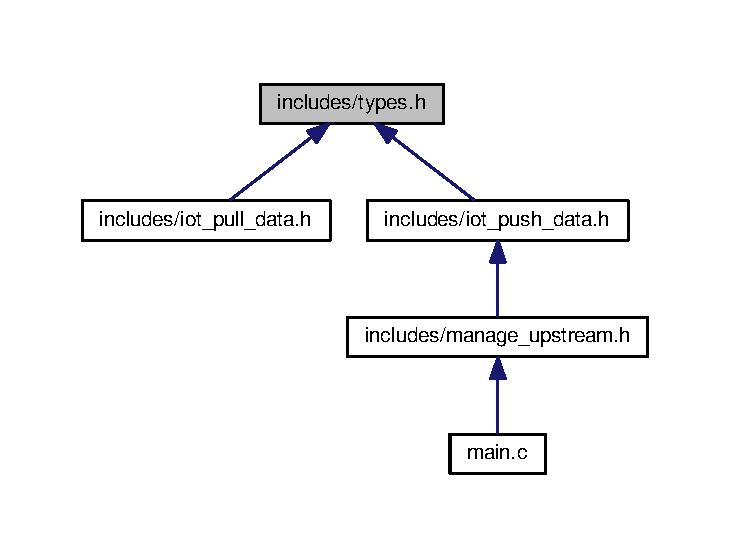
\includegraphics[width=350pt]{types_8h__dep__incl}
\end{center}
\end{figure}
\subsection*{Typedefs}
\begin{DoxyCompactItemize}
\item 
\hypertarget{types_8h_acaed0aa53fc5bf5bbd621d4c1f63dfcc}{typedef int {\bfseries S\-O\-C\-K\-E\-T}}\label{types_8h_acaed0aa53fc5bf5bbd621d4c1f63dfcc}

\item 
\hypertarget{types_8h_a1581cde4f73c9a797ae1e7afcc1bb3de}{typedef unsigned char {\bfseries byte}}\label{types_8h_a1581cde4f73c9a797ae1e7afcc1bb3de}

\end{DoxyCompactItemize}


\subsection{Detailed Description}
This file defines some typedef. \begin{DoxyAuthor}{Author}
Giuliano Franchetto 
\end{DoxyAuthor}
\begin{DoxyDate}{Date}
30/09/2015 
\end{DoxyDate}
\begin{DoxyVersion}{Version}
1 
\end{DoxyVersion}

\hypertarget{main_8c}{\section{main.\-c File Reference}
\label{main_8c}\index{main.\-c@{main.\-c}}
}


This file is the entry of the main program to communicate with the Kerlink Io\-T station.  


{\ttfamily \#include $<$signal.\-h$>$}\\*
{\ttfamily \#include $<$manage\-\_\-upstream.\-h$>$}\\*
{\ttfamily \#include $<$manage\-\_\-downstream.\-h$>$}\\*
Include dependency graph for main.\-c\-:\nopagebreak
\begin{figure}[H]
\begin{center}
\leavevmode
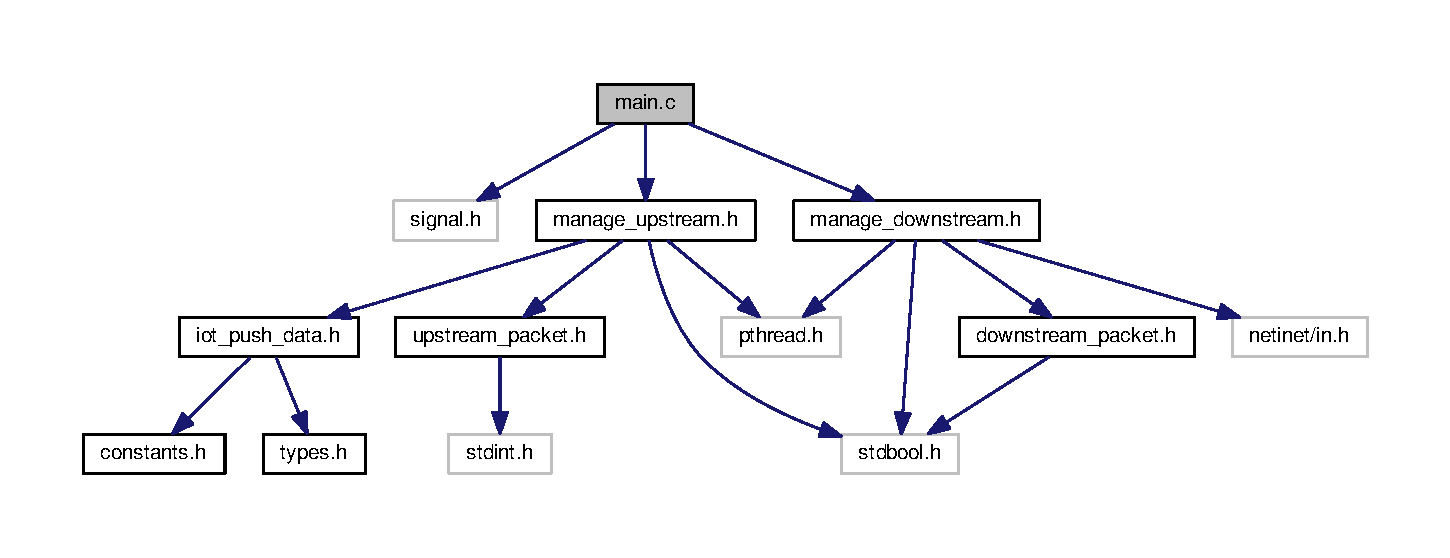
\includegraphics[width=350pt]{main_8c__incl}
\end{center}
\end{figure}
\subsection*{Functions}
\begin{DoxyCompactItemize}
\item 
\hypertarget{main_8c_a427433f28515b38b78316d2c041d06e0}{void {\bfseries signal\-\_\-int} (int sig)}\label{main_8c_a427433f28515b38b78316d2c041d06e0}

\item 
\hypertarget{main_8c_ae66f6b31b5ad750f1fe042a706a4e3d4}{int {\bfseries main} ()}\label{main_8c_ae66f6b31b5ad750f1fe042a706a4e3d4}

\end{DoxyCompactItemize}
\subsection*{Variables}
\begin{DoxyCompactItemize}
\item 
pthread\-\_\-t \hyperlink{main_8c_a49e34dce6ea4518b48454896a6ecd171}{thread\-\_\-manage\-\_\-upstream}
\item 
pthread\-\_\-t \hyperlink{main_8c_a2a9b27e18263ba28e7bf1dda832cff0e}{thread\-\_\-manage\-\_\-downstream}
\item 
bool \hyperlink{main_8c_a4a6f394651f7af3aedb62c255a67bc59}{stop\-\_\-thread\-\_\-upstream} = false
\item 
bool \hyperlink{main_8c_ad54e3fbaaf4a33c07d9a070bf3986a0a}{stop\-\_\-thread\-\_\-downstream} = false
\item 
int \hyperlink{main_8c_a66a09b67a86f445357c6c380f25d1781}{upstream\-\_\-error} = 0
\item 
int \hyperlink{main_8c_a14c8d3b0c27669fa3961afc367df7a77}{downstream\-\_\-error} = 0
\end{DoxyCompactItemize}


\subsection{Detailed Description}
This file is the entry of the main program to communicate with the Kerlink Io\-T station. \begin{DoxyAuthor}{Author}
Giuliano Franchetto 
\end{DoxyAuthor}
\begin{DoxyVersion}{Version}
1.\-0 
\end{DoxyVersion}
\begin{DoxyDate}{Date}
09/30/2015 
\end{DoxyDate}


\subsection{Variable Documentation}
\hypertarget{main_8c_a14c8d3b0c27669fa3961afc367df7a77}{\index{main.\-c@{main.\-c}!downstream\-\_\-error@{downstream\-\_\-error}}
\index{downstream\-\_\-error@{downstream\-\_\-error}!main.c@{main.\-c}}
\subsubsection[{downstream\-\_\-error}]{\setlength{\rightskip}{0pt plus 5cm}int downstream\-\_\-error = 0}}\label{main_8c_a14c8d3b0c27669fa3961afc367df7a77}
The number of error this thread made \hypertarget{main_8c_ad54e3fbaaf4a33c07d9a070bf3986a0a}{\index{main.\-c@{main.\-c}!stop\-\_\-thread\-\_\-downstream@{stop\-\_\-thread\-\_\-downstream}}
\index{stop\-\_\-thread\-\_\-downstream@{stop\-\_\-thread\-\_\-downstream}!main.c@{main.\-c}}
\subsubsection[{stop\-\_\-thread\-\_\-downstream}]{\setlength{\rightskip}{0pt plus 5cm}bool stop\-\_\-thread\-\_\-downstream = false}}\label{main_8c_ad54e3fbaaf4a33c07d9a070bf3986a0a}
A boolean which must set to true to stop the thread \hypertarget{main_8c_a4a6f394651f7af3aedb62c255a67bc59}{\index{main.\-c@{main.\-c}!stop\-\_\-thread\-\_\-upstream@{stop\-\_\-thread\-\_\-upstream}}
\index{stop\-\_\-thread\-\_\-upstream@{stop\-\_\-thread\-\_\-upstream}!main.c@{main.\-c}}
\subsubsection[{stop\-\_\-thread\-\_\-upstream}]{\setlength{\rightskip}{0pt plus 5cm}bool stop\-\_\-thread\-\_\-upstream = false}}\label{main_8c_a4a6f394651f7af3aedb62c255a67bc59}
This varibale must be set to true to stop the thread \hypertarget{main_8c_a2a9b27e18263ba28e7bf1dda832cff0e}{\index{main.\-c@{main.\-c}!thread\-\_\-manage\-\_\-downstream@{thread\-\_\-manage\-\_\-downstream}}
\index{thread\-\_\-manage\-\_\-downstream@{thread\-\_\-manage\-\_\-downstream}!main.c@{main.\-c}}
\subsubsection[{thread\-\_\-manage\-\_\-downstream}]{\setlength{\rightskip}{0pt plus 5cm}pthread\-\_\-t thread\-\_\-manage\-\_\-downstream}}\label{main_8c_a2a9b27e18263ba28e7bf1dda832cff0e}
The pthread\-\_\-t used for the manage\-\_\-downstream thread \hypertarget{main_8c_a49e34dce6ea4518b48454896a6ecd171}{\index{main.\-c@{main.\-c}!thread\-\_\-manage\-\_\-upstream@{thread\-\_\-manage\-\_\-upstream}}
\index{thread\-\_\-manage\-\_\-upstream@{thread\-\_\-manage\-\_\-upstream}!main.c@{main.\-c}}
\subsubsection[{thread\-\_\-manage\-\_\-upstream}]{\setlength{\rightskip}{0pt plus 5cm}pthread\-\_\-t thread\-\_\-manage\-\_\-upstream}}\label{main_8c_a49e34dce6ea4518b48454896a6ecd171}
The thread used by the manage\-\_\-upstream routine \hypertarget{main_8c_a66a09b67a86f445357c6c380f25d1781}{\index{main.\-c@{main.\-c}!upstream\-\_\-error@{upstream\-\_\-error}}
\index{upstream\-\_\-error@{upstream\-\_\-error}!main.c@{main.\-c}}
\subsubsection[{upstream\-\_\-error}]{\setlength{\rightskip}{0pt plus 5cm}int upstream\-\_\-error = 0}}\label{main_8c_a66a09b67a86f445357c6c380f25d1781}
The number of error the upstream thread did 
%--- End generated contents ---

% Index
\newpage
\phantomsection
\addcontentsline{toc}{chapter}{Index}
\printindex

\end{document}
